\documentclass[twoside]{book}

% Packages required by doxygen
\usepackage{fixltx2e}
\usepackage{calc}
\usepackage{doxygen}
\usepackage[export]{adjustbox} % also loads graphicx
\usepackage{graphicx}
\usepackage[utf8]{inputenc}
\usepackage{makeidx}
\usepackage{multicol}
\usepackage{multirow}
\PassOptionsToPackage{warn}{textcomp}
\usepackage{textcomp}
\usepackage[nointegrals]{wasysym}
\usepackage[table]{xcolor}

% Font selection
\usepackage[T1]{fontenc}
\usepackage[scaled=.90]{helvet}
\usepackage{courier}
\usepackage{amssymb}
\usepackage{sectsty}
\renewcommand{\familydefault}{\sfdefault}
\allsectionsfont{%
  \fontseries{bc}\selectfont%
  \color{darkgray}%
}
\renewcommand{\DoxyLabelFont}{%
  \fontseries{bc}\selectfont%
  \color{darkgray}%
}
\newcommand{\+}{\discretionary{\mbox{\scriptsize$\hookleftarrow$}}{}{}}

% Page & text layout
\usepackage{geometry}
\geometry{%
  a4paper,%
  top=2.5cm,%
  bottom=2.5cm,%
  left=2.5cm,%
  right=2.5cm%
}
\tolerance=750
\hfuzz=15pt
\hbadness=750
\setlength{\emergencystretch}{15pt}
\setlength{\parindent}{0cm}
\setlength{\parskip}{3ex plus 2ex minus 2ex}
\makeatletter
\renewcommand{\paragraph}{%
  \@startsection{paragraph}{4}{0ex}{-1.0ex}{1.0ex}{%
    \normalfont\normalsize\bfseries\SS@parafont%
  }%
}
\renewcommand{\subparagraph}{%
  \@startsection{subparagraph}{5}{0ex}{-1.0ex}{1.0ex}{%
    \normalfont\normalsize\bfseries\SS@subparafont%
  }%
}
\makeatother

% Headers & footers
\usepackage{fancyhdr}
\pagestyle{fancyplain}
\fancyhead[LE]{\fancyplain{}{\bfseries\thepage}}
\fancyhead[CE]{\fancyplain{}{}}
\fancyhead[RE]{\fancyplain{}{\bfseries\leftmark}}
\fancyhead[LO]{\fancyplain{}{\bfseries\rightmark}}
\fancyhead[CO]{\fancyplain{}{}}
\fancyhead[RO]{\fancyplain{}{\bfseries\thepage}}
\fancyfoot[LE]{\fancyplain{}{}}
\fancyfoot[CE]{\fancyplain{}{}}
\fancyfoot[RE]{\fancyplain{}{\bfseries\scriptsize Generated by Doxygen }}
\fancyfoot[LO]{\fancyplain{}{\bfseries\scriptsize Generated by Doxygen }}
\fancyfoot[CO]{\fancyplain{}{}}
\fancyfoot[RO]{\fancyplain{}{}}
\renewcommand{\footrulewidth}{0.4pt}
\renewcommand{\chaptermark}[1]{%
  \markboth{#1}{}%
}
\renewcommand{\sectionmark}[1]{%
  \markright{\thesection\ #1}%
}

% Indices & bibliography
\usepackage{natbib}
\usepackage[titles]{tocloft}
\setcounter{tocdepth}{3}
\setcounter{secnumdepth}{5}
\makeindex

% Hyperlinks (required, but should be loaded last)
\usepackage{ifpdf}
\ifpdf
  \usepackage[pdftex,pagebackref=true]{hyperref}
\else
  \usepackage[ps2pdf,pagebackref=true]{hyperref}
\fi
\hypersetup{%
  colorlinks=true,%
  linkcolor=blue,%
  citecolor=blue,%
  unicode%
}

% Custom commands
\newcommand{\clearemptydoublepage}{%
  \newpage{\pagestyle{empty}\cleardoublepage}%
}

\usepackage{caption}
\captionsetup{labelsep=space,justification=centering,font={bf},singlelinecheck=off,skip=4pt,position=top}

%===== C O N T E N T S =====

\begin{document}

% Titlepage & ToC
\hypersetup{pageanchor=false,
             bookmarksnumbered=true,
             pdfencoding=unicode
            }
\pagenumbering{alph}
\begin{titlepage}
\vspace*{7cm}
\begin{center}%
{\Large Rmap I2\+C-\/\+Rain \\[1ex]\large 2 }\\
\vspace*{1cm}
{\large Generated by Doxygen 1.8.13}\\
\end{center}
\end{titlepage}
\clearemptydoublepage
\pagenumbering{roman}
\tableofcontents
\clearemptydoublepage
\pagenumbering{arabic}
\hypersetup{pageanchor=true}

%--- Begin generated contents ---
\chapter{Class Index}
\section{Class List}
Here are the classes, structs, unions and interfaces with brief descriptions\+:\begin{DoxyCompactList}
\item\contentsline{section}{\hyperlink{structconfiguration__t}{configuration\+\_\+t} \\*E\+E\+P\+R\+OM saved configuration }{\pageref{structconfiguration__t}}{}
\end{DoxyCompactList}

\chapter{File Index}
\section{File List}
Here is a list of all documented files with brief descriptions\+:\begin{DoxyCompactList}
\item\contentsline{section}{sketchbook/libraries/\+Digiteco\+Power/\hyperlink{digiteco__power_8cpp}{digiteco\+\_\+power.\+cpp} }{\pageref{digiteco__power_8cpp}}{}
\item\contentsline{section}{sketchbook/libraries/\+Digiteco\+Power/\hyperlink{digiteco__power_8h}{digiteco\+\_\+power.\+h} }{\pageref{digiteco__power_8h}}{}
\item\contentsline{section}{sketchbook/libraries/\+H\+Y\+T2\+X1/\hyperlink{hyt2x1_8cpp}{hyt2x1.\+cpp} }{\pageref{hyt2x1_8cpp}}{}
\item\contentsline{section}{sketchbook/libraries/\+H\+Y\+T2\+X1/\hyperlink{hyt2x1_8h}{hyt2x1.\+h} }{\pageref{hyt2x1_8h}}{}
\item\contentsline{section}{sketchbook/libraries/\+N\+T\+P/\hyperlink{ntp_8cpp}{ntp.\+cpp} }{\pageref{ntp_8cpp}}{}
\item\contentsline{section}{sketchbook/libraries/\+N\+T\+P/\hyperlink{ntp_8h}{ntp.\+h} }{\pageref{ntp_8h}}{}
\item\contentsline{section}{sketchbook/libraries/\+P\+C\+F8563/\hyperlink{pcf8563_8cpp}{pcf8563.\+cpp} }{\pageref{pcf8563_8cpp}}{}
\item\contentsline{section}{sketchbook/libraries/\+P\+C\+F8563/\hyperlink{pcf8563_8h}{pcf8563.\+h} }{\pageref{pcf8563_8h}}{}
\item\contentsline{section}{sketchbook/libraries/\+Rmap/\hyperlink{debug_8cpp}{debug.\+cpp} }{\pageref{debug_8cpp}}{}
\item\contentsline{section}{sketchbook/libraries/\+Rmap/\hyperlink{debug_8h}{debug.\+h} }{\pageref{debug_8h}}{}
\item\contentsline{section}{sketchbook/libraries/\+Rmap/\hyperlink{eeprom__utility_8h}{eeprom\+\_\+utility.\+h} }{\pageref{eeprom__utility_8h}}{}
\item\contentsline{section}{sketchbook/libraries/\+Rmap/\hyperlink{i2c__utility_8cpp}{i2c\+\_\+utility.\+cpp} }{\pageref{i2c__utility_8cpp}}{}
\item\contentsline{section}{sketchbook/libraries/\+Rmap/\hyperlink{i2c__utility_8h}{i2c\+\_\+utility.\+h} }{\pageref{i2c__utility_8h}}{}
\item\contentsline{section}{sketchbook/libraries/\+Rmap/\hyperlink{registers-rain_8h}{registers-\/rain.\+h} }{\pageref{registers-rain_8h}}{}
\item\contentsline{section}{sketchbook/libraries/\+Rmap/\hyperlink{registers-th_8h}{registers-\/th.\+h} }{\pageref{registers-th_8h}}{}
\item\contentsline{section}{sketchbook/libraries/\+Rmap/\hyperlink{registers_8h}{registers.\+h} }{\pageref{registers_8h}}{}
\item\contentsline{section}{sketchbook/libraries/\+Rmap/\hyperlink{rmap__utility_8cpp}{rmap\+\_\+utility.\+cpp} }{\pageref{rmap__utility_8cpp}}{}
\item\contentsline{section}{sketchbook/libraries/\+Rmap/\hyperlink{rmap__utility_8h}{rmap\+\_\+utility.\+h} }{\pageref{rmap__utility_8h}}{}
\item\contentsline{section}{sketchbook/libraries/\+Rmap/\hyperlink{sdcard__utility_8cpp}{sdcard\+\_\+utility.\+cpp} }{\pageref{sdcard__utility_8cpp}}{}
\item\contentsline{section}{sketchbook/libraries/\+Rmap/\hyperlink{sdcard__utility_8h}{sdcard\+\_\+utility.\+h} }{\pageref{sdcard__utility_8h}}{}
\item\contentsline{section}{sketchbook/libraries/\+Rmap/\hyperlink{stima__module_8h}{stima\+\_\+module.\+h} }{\pageref{stima__module_8h}}{}
\item\contentsline{section}{sketchbook/libraries/\+Rmap/\hyperlink{typedef_8h}{typedef.\+h} }{\pageref{typedef_8h}}{}
\item\contentsline{section}{sketchbook/libraries/\+Rmap\+Config/\hyperlink{debug__config_8h}{debug\+\_\+config.\+h} }{\pageref{debug__config_8h}}{}
\item\contentsline{section}{sketchbook/libraries/\+Rmap\+Config/\hyperlink{ethernet__config_8h}{ethernet\+\_\+config.\+h} }{\pageref{ethernet__config_8h}}{}
\item\contentsline{section}{sketchbook/libraries/\+Rmap\+Config/\hyperlink{gsm__config_8h}{gsm\+\_\+config.\+h} }{\pageref{gsm__config_8h}}{}
\item\contentsline{section}{sketchbook/libraries/\+Rmap\+Config/\hyperlink{hardware__config_8h}{hardware\+\_\+config.\+h} }{\pageref{hardware__config_8h}}{}
\item\contentsline{section}{sketchbook/libraries/\+Rmap\+Config/\hyperlink{json__config_8h}{json\+\_\+config.\+h} }{\pageref{json__config_8h}}{}
\item\contentsline{section}{sketchbook/libraries/\+Rmap\+Config/\hyperlink{lcd__config_8h}{lcd\+\_\+config.\+h} }{\pageref{lcd__config_8h}}{}
\item\contentsline{section}{sketchbook/libraries/\+Rmap\+Config/\hyperlink{mqtt__config_8h}{mqtt\+\_\+config.\+h} }{\pageref{mqtt__config_8h}}{}
\item\contentsline{section}{sketchbook/libraries/\+Rmap\+Config/\hyperlink{ntp__config_8h}{ntp\+\_\+config.\+h} }{\pageref{ntp__config_8h}}{}
\item\contentsline{section}{sketchbook/libraries/\+Rmap\+Config/\hyperlink{sdcard__config_8h}{sdcard\+\_\+config.\+h} }{\pageref{sdcard__config_8h}}{}
\item\contentsline{section}{sketchbook/libraries/\+Rmap\+Config/\hyperlink{sensors__config_8h}{sensors\+\_\+config.\+h} }{\pageref{sensors__config_8h}}{}
\item\contentsline{section}{sketchbook/libraries/\+Sensor\+Driver/\hyperlink{SensorDriver_8cpp}{Sensor\+Driver.\+cpp} }{\pageref{SensorDriver_8cpp}}{}
\item\contentsline{section}{sketchbook/libraries/\+Sensor\+Driver/\hyperlink{SensorDriver_8h}{Sensor\+Driver.\+h} }{\pageref{SensorDriver_8h}}{}
\item\contentsline{section}{sketchbook/libraries/\+Sensor\+Driver/\hyperlink{SensorDriverSensors_8h}{Sensor\+Driver\+Sensors.\+h} }{\pageref{SensorDriverSensors_8h}}{}
\item\contentsline{section}{sketchbook/libraries/sim800/\hyperlink{sim800_8cpp}{sim800.\+cpp} }{\pageref{sim800_8cpp}}{}
\item\contentsline{section}{sketchbook/libraries/sim800/\hyperlink{sim800_8h}{sim800.\+h} }{\pageref{sim800_8h}}{}
\item\contentsline{section}{sketchbook/libraries/sim800/\hyperlink{sim800Client_8h}{sim800\+Client.\+h} }{\pageref{sim800Client_8h}}{}
\item\contentsline{section}{sketchbook/rmap/{\bfseries version.\+h} }{\pageref{version_8h}}{}
\item\contentsline{section}{sketchbook/rmap/i2c-\/rain/\hyperlink{i2c-rain-config_8h}{i2c-\/rain-\/config.\+h} }{\pageref{i2c-rain-config_8h}}{}
\item\contentsline{section}{sketchbook/rmap/i2c-\/rain/\hyperlink{i2c-rain_8h}{i2c-\/rain.\+h} }{\pageref{i2c-rain_8h}}{}
\item\contentsline{section}{sketchbook/rmap/i2c-\/rain/\hyperlink{i2c-rain_8ino}{i2c-\/rain.\+ino} }{\pageref{i2c-rain_8ino}}{}
\item\contentsline{section}{sketchbook/rmap/i2c-\/th/\hyperlink{i2c-th-config_8h}{i2c-\/th-\/config.\+h} }{\pageref{i2c-th-config_8h}}{}
\item\contentsline{section}{sketchbook/rmap/i2c-\/th/\hyperlink{i2c-th_8h}{i2c-\/th.\+h} }{\pageref{i2c-th_8h}}{}
\item\contentsline{section}{sketchbook/rmap/i2c-\/th/\hyperlink{i2c-th_8ino}{i2c-\/th.\+ino} }{\pageref{i2c-th_8ino}}{}
\item\contentsline{section}{sketchbook/rmap/rmap/\hyperlink{rmap-config_8h}{rmap-\/config.\+h} }{\pageref{rmap-config_8h}}{}
\item\contentsline{section}{sketchbook/rmap/rmap/\hyperlink{rmap_8h}{rmap.\+h} }{\pageref{rmap_8h}}{}
\item\contentsline{section}{sketchbook/rmap/rmap/\hyperlink{rmap_8ino}{rmap.\+ino} }{\pageref{rmap_8ino}}{}
\end{DoxyCompactList}

\chapter{Class Documentation}
\hypertarget{structconfiguration__t}{}\section{configuration\+\_\+t Struct Reference}
\label{structconfiguration__t}\index{configuration\+\_\+t@{configuration\+\_\+t}}


E\+E\+P\+R\+OM saved configuration.  




{\ttfamily \#include $<$i2c-\/rain.\+h$>$}



Collaboration diagram for configuration\+\_\+t\+:\nopagebreak
\begin{figure}[H]
\begin{center}
\leavevmode
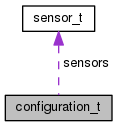
\includegraphics[width=160pt]{structconfiguration__t__coll__graph}
\end{center}
\end{figure}
\subsection*{Public Attributes}
\begin{DoxyCompactItemize}
\item 
\mbox{\Hypertarget{structconfiguration__t_a32d4c4bb78b5b231704c8a9f8d1b9e87}\label{structconfiguration__t_a32d4c4bb78b5b231704c8a9f8d1b9e87}} 
uint8\+\_\+t \hyperlink{structconfiguration__t_a32d4c4bb78b5b231704c8a9f8d1b9e87}{module\+\_\+version}
\begin{DoxyCompactList}\small\item\em module version \end{DoxyCompactList}\item 
\mbox{\Hypertarget{structconfiguration__t_a7dab895a0a9aa44bb65d90ef8016127d}\label{structconfiguration__t_a7dab895a0a9aa44bb65d90ef8016127d}} 
uint8\+\_\+t \hyperlink{structconfiguration__t_a7dab895a0a9aa44bb65d90ef8016127d}{module\+\_\+type}
\begin{DoxyCompactList}\small\item\em module type \end{DoxyCompactList}\item 
\mbox{\Hypertarget{structconfiguration__t_a0e088540266e347426ae73aed159f63a}\label{structconfiguration__t_a0e088540266e347426ae73aed159f63a}} 
uint8\+\_\+t \hyperlink{structconfiguration__t_a0e088540266e347426ae73aed159f63a}{i2c\+\_\+address}
\begin{DoxyCompactList}\small\item\em i2c address \end{DoxyCompactList}\item 
\mbox{\Hypertarget{structconfiguration__t_a227ef462f171f25e31cb3b0ce70b2597}\label{structconfiguration__t_a227ef462f171f25e31cb3b0ce70b2597}} 
bool \hyperlink{structconfiguration__t_a227ef462f171f25e31cb3b0ce70b2597}{is\+\_\+oneshot}
\begin{DoxyCompactList}\small\item\em enable or disable oneshot mode \end{DoxyCompactList}\item 
\mbox{\Hypertarget{structconfiguration__t_a33f99299576a58b3eb55be371e143531}\label{structconfiguration__t_a33f99299576a58b3eb55be371e143531}} 
bool \hyperlink{structconfiguration__t_a33f99299576a58b3eb55be371e143531}{is\+\_\+continuous}
\begin{DoxyCompactList}\small\item\em enable or disable continuous mode \end{DoxyCompactList}\item 
\mbox{\Hypertarget{structconfiguration__t_aed0a51c0dfbd925368c8539cf10c3001}\label{structconfiguration__t_aed0a51c0dfbd925368c8539cf10c3001}} 
uint8\+\_\+t \hyperlink{structconfiguration__t_aed0a51c0dfbd925368c8539cf10c3001}{i2c\+\_\+temperature\+\_\+address}
\begin{DoxyCompactList}\small\item\em i2c address of temperature sensor \end{DoxyCompactList}\item 
\mbox{\Hypertarget{structconfiguration__t_a79d1b1d9cb095c2bc0deb36c4f44452c}\label{structconfiguration__t_a79d1b1d9cb095c2bc0deb36c4f44452c}} 
uint8\+\_\+t \hyperlink{structconfiguration__t_a79d1b1d9cb095c2bc0deb36c4f44452c}{i2c\+\_\+humidity\+\_\+address}
\begin{DoxyCompactList}\small\item\em i2c address of humidity sensor \end{DoxyCompactList}\item 
\mbox{\Hypertarget{structconfiguration__t_aa003a99852a65bd2f9de0d230568bbbf}\label{structconfiguration__t_aa003a99852a65bd2f9de0d230568bbbf}} 
uint16\+\_\+t \hyperlink{structconfiguration__t_aa003a99852a65bd2f9de0d230568bbbf}{mqtt\+\_\+port}
\begin{DoxyCompactList}\small\item\em mqtt server port \end{DoxyCompactList}\item 
\mbox{\Hypertarget{structconfiguration__t_ad9a71a593cd2191ed132f9a2d6c00679}\label{structconfiguration__t_ad9a71a593cd2191ed132f9a2d6c00679}} 
char \hyperlink{structconfiguration__t_ad9a71a593cd2191ed132f9a2d6c00679}{mqtt\+\_\+server} \mbox{[}\hyperlink{mqtt__config_8h_a0a37bcf35cdbfc63d72beca198759c08}{M\+Q\+T\+T\+\_\+\+S\+E\+R\+V\+E\+R\+\_\+\+L\+E\+N\+G\+TH}\mbox{]}
\begin{DoxyCompactList}\small\item\em mqtt server \end{DoxyCompactList}\item 
\mbox{\Hypertarget{structconfiguration__t_acebf92623ad7bdf44f9707b0d99f50da}\label{structconfiguration__t_acebf92623ad7bdf44f9707b0d99f50da}} 
char \hyperlink{structconfiguration__t_acebf92623ad7bdf44f9707b0d99f50da}{mqtt\+\_\+root\+\_\+topic} \mbox{[}\hyperlink{mqtt__config_8h_a6d3b5b0f9c41b605e608f7d460491be6}{M\+Q\+T\+T\+\_\+\+R\+O\+O\+T\+\_\+\+T\+O\+P\+I\+C\+\_\+\+L\+E\+N\+G\+TH}\mbox{]}
\begin{DoxyCompactList}\small\item\em mqtt root path \end{DoxyCompactList}\item 
\mbox{\Hypertarget{structconfiguration__t_ae3699c4dd6979713472062bbad82c542}\label{structconfiguration__t_ae3699c4dd6979713472062bbad82c542}} 
char \hyperlink{structconfiguration__t_ae3699c4dd6979713472062bbad82c542}{mqtt\+\_\+subscribe\+\_\+topic} \mbox{[}\hyperlink{mqtt__config_8h_a2517f6560f7ee99813533e63d7fc91b6}{M\+Q\+T\+T\+\_\+\+S\+U\+B\+S\+C\+R\+I\+B\+E\+\_\+\+T\+O\+P\+I\+C\+\_\+\+L\+E\+N\+G\+TH}\mbox{]}
\begin{DoxyCompactList}\small\item\em mqtt subscribe topic \end{DoxyCompactList}\item 
\mbox{\Hypertarget{structconfiguration__t_ad97d47b585071f095a97296fc3e260e7}\label{structconfiguration__t_ad97d47b585071f095a97296fc3e260e7}} 
char \hyperlink{structconfiguration__t_ad97d47b585071f095a97296fc3e260e7}{mqtt\+\_\+username} \mbox{[}\hyperlink{mqtt__config_8h_a0e1860b8d036f571ffcb7e6d27832c16}{M\+Q\+T\+T\+\_\+\+U\+S\+E\+R\+N\+A\+M\+E\+\_\+\+L\+E\+N\+G\+TH}\mbox{]}
\begin{DoxyCompactList}\small\item\em mqtt username \end{DoxyCompactList}\item 
\mbox{\Hypertarget{structconfiguration__t_af842b7c625c3fdfb1b810e24fc1ba1b8}\label{structconfiguration__t_af842b7c625c3fdfb1b810e24fc1ba1b8}} 
char \hyperlink{structconfiguration__t_af842b7c625c3fdfb1b810e24fc1ba1b8}{mqtt\+\_\+password} \mbox{[}\hyperlink{mqtt__config_8h_a9fa040018ffd349e846cec27b2791fde}{M\+Q\+T\+T\+\_\+\+P\+A\+S\+S\+W\+O\+R\+D\+\_\+\+L\+E\+N\+G\+TH}\mbox{]}
\begin{DoxyCompactList}\small\item\em mqtt password \end{DoxyCompactList}\item 
\mbox{\Hypertarget{structconfiguration__t_a8de58dc10dfc6b369f34bae82426be5d}\label{structconfiguration__t_a8de58dc10dfc6b369f34bae82426be5d}} 
char \hyperlink{structconfiguration__t_a8de58dc10dfc6b369f34bae82426be5d}{ntp\+\_\+server} \mbox{[}\hyperlink{ntp__config_8h_a54153a6aa87c606f585ab167661b1be2}{N\+T\+P\+\_\+\+S\+E\+R\+V\+E\+R\+\_\+\+L\+E\+N\+G\+TH}\mbox{]}
\begin{DoxyCompactList}\small\item\em ntp server \end{DoxyCompactList}\item 
\mbox{\Hypertarget{structconfiguration__t_adede74f3da6d26f5bc4b5e64e4776f7f}\label{structconfiguration__t_adede74f3da6d26f5bc4b5e64e4776f7f}} 
\hyperlink{structsensor__t}{sensor\+\_\+t} \hyperlink{structconfiguration__t_adede74f3da6d26f5bc4b5e64e4776f7f}{sensors} \mbox{[}\hyperlink{rmap-config_8h_af18dc3de744722cb308451b7a705611b}{U\+S\+E\+\_\+\+S\+E\+N\+S\+O\+R\+S\+\_\+\+C\+O\+U\+NT}\mbox{]}
\begin{DoxyCompactList}\small\item\em \hyperlink{classSensorDriver}{Sensor\+Driver} buffer for storing sensors parameter. \end{DoxyCompactList}\item 
\mbox{\Hypertarget{structconfiguration__t_a9a1e7c702c2dd7270f31aca29264db86}\label{structconfiguration__t_a9a1e7c702c2dd7270f31aca29264db86}} 
uint8\+\_\+t \hyperlink{structconfiguration__t_a9a1e7c702c2dd7270f31aca29264db86}{sensors\+\_\+count}
\begin{DoxyCompactList}\small\item\em configured sensors number \end{DoxyCompactList}\item 
\mbox{\Hypertarget{structconfiguration__t_a0c0dc512cf86464d2e8dad486e042c5c}\label{structconfiguration__t_a0c0dc512cf86464d2e8dad486e042c5c}} 
uint16\+\_\+t \hyperlink{structconfiguration__t_a0c0dc512cf86464d2e8dad486e042c5c}{report\+\_\+seconds}
\begin{DoxyCompactList}\small\item\em seconds for report values \end{DoxyCompactList}\item 
\mbox{\Hypertarget{structconfiguration__t_a04554256dd43582433092cd70dd8b87d}\label{structconfiguration__t_a04554256dd43582433092cd70dd8b87d}} 
bool \hyperlink{structconfiguration__t_a04554256dd43582433092cd70dd8b87d}{is\+\_\+dhcp\+\_\+enable}
\begin{DoxyCompactList}\small\item\em dhcp status \end{DoxyCompactList}\item 
\mbox{\Hypertarget{structconfiguration__t_a6ade77826c87e62532cae8ca0f045dac}\label{structconfiguration__t_a6ade77826c87e62532cae8ca0f045dac}} 
uint8\+\_\+t \hyperlink{structconfiguration__t_a6ade77826c87e62532cae8ca0f045dac}{ethernet\+\_\+mac} \mbox{[}\hyperlink{ethernet__config_8h_aafad911924144dbfc03b66b146ed4439}{E\+T\+H\+E\+R\+N\+E\+T\+\_\+\+M\+A\+C\+\_\+\+L\+E\+N\+G\+TH}\mbox{]}
\begin{DoxyCompactList}\small\item\em ethernet mac \end{DoxyCompactList}\item 
\mbox{\Hypertarget{structconfiguration__t_a0b698acfbb52f889c906b9b175f7a5d5}\label{structconfiguration__t_a0b698acfbb52f889c906b9b175f7a5d5}} 
uint8\+\_\+t \hyperlink{structconfiguration__t_a0b698acfbb52f889c906b9b175f7a5d5}{ip} \mbox{[}\hyperlink{ethernet__config_8h_ae8de53528e88d8ff4516d82a48590bd7}{E\+T\+H\+E\+R\+N\+E\+T\+\_\+\+I\+P\+\_\+\+L\+E\+N\+G\+TH}\mbox{]}
\begin{DoxyCompactList}\small\item\em ip address \end{DoxyCompactList}\item 
\mbox{\Hypertarget{structconfiguration__t_a60716ed8c6a82119a46eb6345b88ca32}\label{structconfiguration__t_a60716ed8c6a82119a46eb6345b88ca32}} 
uint8\+\_\+t \hyperlink{structconfiguration__t_a60716ed8c6a82119a46eb6345b88ca32}{netmask} \mbox{[}\hyperlink{ethernet__config_8h_ae8de53528e88d8ff4516d82a48590bd7}{E\+T\+H\+E\+R\+N\+E\+T\+\_\+\+I\+P\+\_\+\+L\+E\+N\+G\+TH}\mbox{]}
\begin{DoxyCompactList}\small\item\em netmask \end{DoxyCompactList}\item 
\mbox{\Hypertarget{structconfiguration__t_a9d18b7f4094f4d7a50d2245e0370adc0}\label{structconfiguration__t_a9d18b7f4094f4d7a50d2245e0370adc0}} 
uint8\+\_\+t \hyperlink{structconfiguration__t_a9d18b7f4094f4d7a50d2245e0370adc0}{gateway} \mbox{[}\hyperlink{ethernet__config_8h_ae8de53528e88d8ff4516d82a48590bd7}{E\+T\+H\+E\+R\+N\+E\+T\+\_\+\+I\+P\+\_\+\+L\+E\+N\+G\+TH}\mbox{]}
\begin{DoxyCompactList}\small\item\em gateway \end{DoxyCompactList}\item 
\mbox{\Hypertarget{structconfiguration__t_acd481c434576a90959c342e877985b32}\label{structconfiguration__t_acd481c434576a90959c342e877985b32}} 
uint8\+\_\+t \hyperlink{structconfiguration__t_acd481c434576a90959c342e877985b32}{primary\+\_\+dns} \mbox{[}\hyperlink{ethernet__config_8h_ae8de53528e88d8ff4516d82a48590bd7}{E\+T\+H\+E\+R\+N\+E\+T\+\_\+\+I\+P\+\_\+\+L\+E\+N\+G\+TH}\mbox{]}
\begin{DoxyCompactList}\small\item\em primary dns \end{DoxyCompactList}\end{DoxyCompactItemize}


\subsection{Detailed Description}
E\+E\+P\+R\+OM saved configuration. 

The documentation for this struct was generated from the following files\+:\begin{DoxyCompactItemize}
\item 
sketchbook/rmap/i2c-\/rain/\hyperlink{i2c-rain_8h}{i2c-\/rain.\+h}\item 
sketchbook/rmap/i2c-\/th/\hyperlink{i2c-th_8h}{i2c-\/th.\+h}\item 
sketchbook/rmap/rmap/\hyperlink{rmap_8h}{rmap.\+h}\end{DoxyCompactItemize}

\hypertarget{structreadable__data__t}{}\section{readable\+\_\+data\+\_\+t Struct Reference}
\label{structreadable__data__t}\index{readable\+\_\+data\+\_\+t@{readable\+\_\+data\+\_\+t}}


Readable data through i2c bus.  




{\ttfamily \#include $<$i2c-\/rain.\+h$>$}



Collaboration diagram for readable\+\_\+data\+\_\+t\+:\nopagebreak
\begin{figure}[H]
\begin{center}
\leavevmode
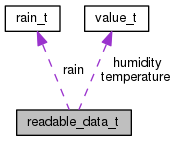
\includegraphics[width=204pt]{structreadable__data__t__coll__graph}
\end{center}
\end{figure}
\subsection*{Public Attributes}
\begin{DoxyCompactItemize}
\item 
\mbox{\Hypertarget{structreadable__data__t_a650c71ad521e965abe34eafda7cf872d}\label{structreadable__data__t_a650c71ad521e965abe34eafda7cf872d}} 
uint8\+\_\+t \hyperlink{structreadable__data__t_a650c71ad521e965abe34eafda7cf872d}{module\+\_\+type}
\begin{DoxyCompactList}\small\item\em module version \end{DoxyCompactList}\item 
\mbox{\Hypertarget{structreadable__data__t_a0b5fa5d2d89bef1b53036512525127f0}\label{structreadable__data__t_a0b5fa5d2d89bef1b53036512525127f0}} 
uint8\+\_\+t \hyperlink{structreadable__data__t_a0b5fa5d2d89bef1b53036512525127f0}{module\+\_\+version}
\begin{DoxyCompactList}\small\item\em module type \end{DoxyCompactList}\item 
\mbox{\Hypertarget{structreadable__data__t_a183ab6eb973fe8deb1c6d0583a991e92}\label{structreadable__data__t_a183ab6eb973fe8deb1c6d0583a991e92}} 
\hyperlink{structrain__t}{rain\+\_\+t} \hyperlink{structreadable__data__t_a183ab6eb973fe8deb1c6d0583a991e92}{rain}
\begin{DoxyCompactList}\small\item\em rain data \end{DoxyCompactList}\item 
\mbox{\Hypertarget{structreadable__data__t_a5852a1cd826e865b18a07fa4be784c6d}\label{structreadable__data__t_a5852a1cd826e865b18a07fa4be784c6d}} 
\hyperlink{structvalue__t}{value\+\_\+t} \hyperlink{structreadable__data__t_a5852a1cd826e865b18a07fa4be784c6d}{temperature}
\begin{DoxyCompactList}\small\item\em temperature data for report \end{DoxyCompactList}\item 
\mbox{\Hypertarget{structreadable__data__t_ab296c803ef271e46364679c955711e26}\label{structreadable__data__t_ab296c803ef271e46364679c955711e26}} 
\hyperlink{structvalue__t}{value\+\_\+t} \hyperlink{structreadable__data__t_ab296c803ef271e46364679c955711e26}{humidity}
\begin{DoxyCompactList}\small\item\em humidity data for report \end{DoxyCompactList}\end{DoxyCompactItemize}


\subsection{Detailed Description}
Readable data through i2c bus. 

The documentation for this struct was generated from the following files\+:\begin{DoxyCompactItemize}
\item 
sketchbook/rmap/i2c-\/rain/\hyperlink{i2c-rain_8h}{i2c-\/rain.\+h}\item 
sketchbook/rmap/i2c-\/th/\hyperlink{i2c-th_8h}{i2c-\/th.\+h}\end{DoxyCompactItemize}

\hypertarget{structwritable__data__t}{}\section{writable\+\_\+data\+\_\+t Struct Reference}
\label{structwritable__data__t}\index{writable\+\_\+data\+\_\+t@{writable\+\_\+data\+\_\+t}}


Writable data through i2c bus.  




{\ttfamily \#include $<$i2c-\/th.\+h$>$}

\subsection*{Public Attributes}
\begin{DoxyCompactItemize}
\item 
\mbox{\Hypertarget{structwritable__data__t_a539304e9f0f30b03691af8b1e8cb6a16}\label{structwritable__data__t_a539304e9f0f30b03691af8b1e8cb6a16}} 
uint8\+\_\+t \hyperlink{structwritable__data__t_a539304e9f0f30b03691af8b1e8cb6a16}{i2c\+\_\+address}
\begin{DoxyCompactList}\small\item\em i2c address \end{DoxyCompactList}\item 
\mbox{\Hypertarget{structwritable__data__t_afc3c86659df5f3a0840313702c7f66fe}\label{structwritable__data__t_afc3c86659df5f3a0840313702c7f66fe}} 
bool \hyperlink{structwritable__data__t_afc3c86659df5f3a0840313702c7f66fe}{is\+\_\+oneshot}
\begin{DoxyCompactList}\small\item\em enable or disable oneshot mode \end{DoxyCompactList}\item 
\mbox{\Hypertarget{structwritable__data__t_a9c3b7927d969d6f21fe475fd3d67f485}\label{structwritable__data__t_a9c3b7927d969d6f21fe475fd3d67f485}} 
bool \hyperlink{structwritable__data__t_a9c3b7927d969d6f21fe475fd3d67f485}{is\+\_\+continuous}
\begin{DoxyCompactList}\small\item\em enable or disable continuous mode \end{DoxyCompactList}\item 
\mbox{\Hypertarget{structwritable__data__t_ad1852e6418870b503cc307a106aff52e}\label{structwritable__data__t_ad1852e6418870b503cc307a106aff52e}} 
uint8\+\_\+t \hyperlink{structwritable__data__t_ad1852e6418870b503cc307a106aff52e}{i2c\+\_\+temperature\+\_\+address}
\begin{DoxyCompactList}\small\item\em i2c address of temperature sensor \end{DoxyCompactList}\item 
\mbox{\Hypertarget{structwritable__data__t_af7dee4cff91376d89745a86ba747c35f}\label{structwritable__data__t_af7dee4cff91376d89745a86ba747c35f}} 
uint8\+\_\+t \hyperlink{structwritable__data__t_af7dee4cff91376d89745a86ba747c35f}{i2c\+\_\+humidity\+\_\+address}
\begin{DoxyCompactList}\small\item\em i2c address of humidity sensor \end{DoxyCompactList}\end{DoxyCompactItemize}


\subsection{Detailed Description}
Writable data through i2c bus. 

The documentation for this struct was generated from the following file\+:\begin{DoxyCompactItemize}
\item 
\hyperlink{i2c-th_8h}{i2c-\/th.\+h}\end{DoxyCompactItemize}

\chapter{File Documentation}
\hypertarget{i2c-rain-config_8h}{}\section{sketchbook/rmap/i2c-\/rain/i2c-\/rain-\/config.h File Reference}
\label{i2c-rain-config_8h}\index{sketchbook/rmap/i2c-\/rain/i2c-\/rain-\/config.\+h@{sketchbook/rmap/i2c-\/rain/i2c-\/rain-\/config.\+h}}
{\ttfamily \#include $<$sensors\+\_\+config.\+h$>$}\newline
Include dependency graph for i2c-\/rain-\/config.h\+:\nopagebreak
\begin{figure}[H]
\begin{center}
\leavevmode
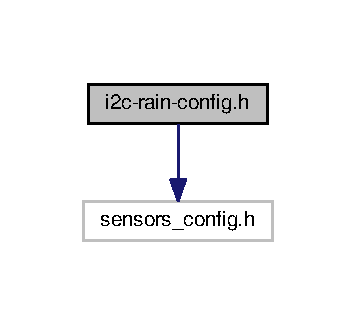
\includegraphics[width=187pt]{i2c-rain-config_8h__incl}
\end{center}
\end{figure}
This graph shows which files directly or indirectly include this file\+:\nopagebreak
\begin{figure}[H]
\begin{center}
\leavevmode
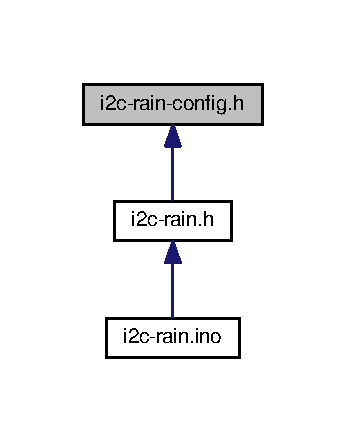
\includegraphics[width=187pt]{i2c-rain-config_8h__dep__incl}
\end{center}
\end{figure}
\subsection*{Macros}
\begin{DoxyCompactItemize}
\item 
\mbox{\Hypertarget{i2c-rain-config_8h_aa8639a8d4e83d9cc4187d7a751228464}\label{i2c-rain-config_8h_aa8639a8d4e83d9cc4187d7a751228464}} 
\#define \hyperlink{i2c-rain-config_8h_aa8639a8d4e83d9cc4187d7a751228464}{M\+O\+D\+U\+L\+E\+\_\+\+V\+E\+R\+S\+I\+ON}~(3)
\begin{DoxyCompactList}\small\item\em Module version. \end{DoxyCompactList}\item 
\mbox{\Hypertarget{i2c-rain-config_8h_a8c815d03b3fd3e18ca06f920a1eb4e8e}\label{i2c-rain-config_8h_a8c815d03b3fd3e18ca06f920a1eb4e8e}} 
\#define \hyperlink{i2c-rain-config_8h_a8c815d03b3fd3e18ca06f920a1eb4e8e}{M\+O\+D\+U\+L\+E\+\_\+\+T\+Y\+PE}~(\hyperlink{stima__module_8h_a4943971f8bec57e337e3f40f085b7fa3}{S\+T\+I\+M\+A\+\_\+\+M\+O\+D\+U\+L\+E\+\_\+\+T\+Y\+P\+E\+\_\+\+R\+A\+IN})
\begin{DoxyCompactList}\small\item\em Type of module. It is defined in \hyperlink{registers_8h}{registers.\+h}. \end{DoxyCompactList}\item 
\mbox{\Hypertarget{i2c-rain-config_8h_a1023d789b828a59d3d22b2c1dddf5702}\label{i2c-rain-config_8h_a1023d789b828a59d3d22b2c1dddf5702}} 
\#define \hyperlink{i2c-rain-config_8h_a1023d789b828a59d3d22b2c1dddf5702}{T\+I\+P\+P\+I\+N\+G\+\_\+\+B\+U\+C\+K\+E\+T\+\_\+\+P\+IN}~(2)
\begin{DoxyCompactList}\small\item\em Interrupt pin for tipping bucket rain gauge. \end{DoxyCompactList}\item 
\mbox{\Hypertarget{i2c-rain-config_8h_a96fb36600c0cea5d22644c26e2d1c7e8}\label{i2c-rain-config_8h_a96fb36600c0cea5d22644c26e2d1c7e8}} 
\#define \hyperlink{i2c-rain-config_8h_a96fb36600c0cea5d22644c26e2d1c7e8}{D\+E\+B\+O\+U\+N\+C\+I\+N\+G\+\_\+\+T\+I\+P\+P\+I\+N\+G\+\_\+\+B\+U\+C\+K\+E\+T\+\_\+\+T\+I\+M\+E\+\_\+\+MS}~(200)
\begin{DoxyCompactList}\small\item\em Debouncing tipping bucket time in milliseconds. \end{DoxyCompactList}\item 
\mbox{\Hypertarget{i2c-rain-config_8h_a5c4024778a87026713c77babd50c06e8}\label{i2c-rain-config_8h_a5c4024778a87026713c77babd50c06e8}} 
\#define \hyperlink{i2c-rain-config_8h_a5c4024778a87026713c77babd50c06e8}{C\+O\+N\+F\+I\+G\+U\+R\+A\+T\+I\+O\+N\+\_\+\+D\+E\+F\+A\+U\+L\+T\+\_\+\+I\+S\+\_\+\+O\+N\+E\+S\+H\+OT}~(true)
\begin{DoxyCompactList}\small\item\em Oneshot mode for default. \end{DoxyCompactList}\item 
\mbox{\Hypertarget{i2c-rain-config_8h_a21819dc42c8c71731e30c99bcf8b0f76}\label{i2c-rain-config_8h_a21819dc42c8c71731e30c99bcf8b0f76}} 
\#define \hyperlink{i2c-rain-config_8h_a21819dc42c8c71731e30c99bcf8b0f76}{C\+O\+N\+F\+I\+G\+U\+R\+A\+T\+I\+O\+N\+\_\+\+D\+E\+F\+A\+U\+L\+T\+\_\+\+I\+S\+\_\+\+C\+O\+N\+T\+I\+N\+U\+O\+US}~(false)
\begin{DoxyCompactList}\small\item\em Continuous mode for default. \end{DoxyCompactList}\item 
\mbox{\Hypertarget{i2c-rain-config_8h_a25fb304ef264a84353f1d4cfc61128e9}\label{i2c-rain-config_8h_a25fb304ef264a84353f1d4cfc61128e9}} 
\#define \hyperlink{i2c-rain-config_8h_a25fb304ef264a84353f1d4cfc61128e9}{C\+O\+N\+F\+I\+G\+U\+R\+A\+T\+I\+O\+N\+\_\+\+D\+E\+F\+A\+U\+L\+T\+\_\+\+I2\+C\+\_\+\+A\+D\+D\+R\+E\+SS}~(\hyperlink{registers-rain_8h_a2aebb0ca4cdf424c57dee6f591c40e0c}{I2\+C\+\_\+\+R\+A\+I\+N\+\_\+\+D\+E\+F\+A\+U\+L\+T\+\_\+\+A\+D\+D\+R\+E\+SS})
\begin{DoxyCompactList}\small\item\em Default i2c address. \end{DoxyCompactList}\item 
\mbox{\Hypertarget{i2c-rain-config_8h_ae90da4786d4ba14563681879dba4d39c}\label{i2c-rain-config_8h_ae90da4786d4ba14563681879dba4d39c}} 
\#define \hyperlink{i2c-rain-config_8h_ae90da4786d4ba14563681879dba4d39c}{C\+O\+N\+F\+I\+G\+U\+R\+A\+T\+I\+O\+N\+\_\+\+R\+E\+S\+E\+T\+\_\+\+P\+IN}~(8)
\begin{DoxyCompactList}\small\item\em Input pin for reset configuration at startup. \end{DoxyCompactList}\item 
\mbox{\Hypertarget{i2c-rain-config_8h_a9ace81994cbeb6153f9dd5adf0e6dbee}\label{i2c-rain-config_8h_a9ace81994cbeb6153f9dd5adf0e6dbee}} 
\#define \hyperlink{i2c-rain-config_8h_a9ace81994cbeb6153f9dd5adf0e6dbee}{U\+S\+E\+\_\+\+P\+O\+W\+E\+R\+\_\+\+D\+O\+WN}~(true)
\begin{DoxyCompactList}\small\item\em Enable or disable power down. \end{DoxyCompactList}\item 
\mbox{\Hypertarget{i2c-rain-config_8h_a7b9497e328b8f872cd7677cfd02bbf65}\label{i2c-rain-config_8h_a7b9497e328b8f872cd7677cfd02bbf65}} 
\#define \hyperlink{i2c-rain-config_8h_a7b9497e328b8f872cd7677cfd02bbf65}{D\+E\+B\+O\+U\+N\+C\+I\+N\+G\+\_\+\+P\+O\+W\+E\+R\+\_\+\+D\+O\+W\+N\+\_\+\+T\+I\+M\+E\+\_\+\+MS}~(\hyperlink{i2c-rain-config_8h_a96fb36600c0cea5d22644c26e2d1c7e8}{D\+E\+B\+O\+U\+N\+C\+I\+N\+G\+\_\+\+T\+I\+P\+P\+I\+N\+G\+\_\+\+B\+U\+C\+K\+E\+T\+\_\+\+T\+I\+M\+E\+\_\+\+MS} + 10)
\begin{DoxyCompactList}\small\item\em Debounce power down ms. \end{DoxyCompactList}\item 
\mbox{\Hypertarget{i2c-rain-config_8h_a8051c2a569a9f9c488af89bce47ec306}\label{i2c-rain-config_8h_a8051c2a569a9f9c488af89bce47ec306}} 
\#define \hyperlink{i2c-rain-config_8h_a8051c2a569a9f9c488af89bce47ec306}{U\+S\+E\+\_\+\+T\+I\+M\+E\+R\+\_\+1}~(false)
\begin{DoxyCompactList}\small\item\em Enable or disable timer1. \end{DoxyCompactList}\item 
\#define \hyperlink{i2c-rain-config_8h_a983c9777673ee873f12ec9f489215321}{W\+D\+T\+\_\+\+T\+I\+M\+ER}~(W\+D\+T\+O\+\_\+4S)
\begin{DoxyCompactList}\small\item\em Watchdog timer for periodically check microprocessor block states. \end{DoxyCompactList}\end{DoxyCompactItemize}


\subsection{Macro Definition Documentation}
\mbox{\Hypertarget{i2c-rain-config_8h_a983c9777673ee873f12ec9f489215321}\label{i2c-rain-config_8h_a983c9777673ee873f12ec9f489215321}} 
\index{i2c-\/rain-\/config.\+h@{i2c-\/rain-\/config.\+h}!W\+D\+T\+\_\+\+T\+I\+M\+ER@{W\+D\+T\+\_\+\+T\+I\+M\+ER}}
\index{W\+D\+T\+\_\+\+T\+I\+M\+ER@{W\+D\+T\+\_\+\+T\+I\+M\+ER}!i2c-\/rain-\/config.\+h@{i2c-\/rain-\/config.\+h}}
\subsubsection{\texorpdfstring{W\+D\+T\+\_\+\+T\+I\+M\+ER}{WDT\_TIMER}}
{\footnotesize\ttfamily \#define W\+D\+T\+\_\+\+T\+I\+M\+ER~(W\+D\+T\+O\+\_\+4S)}



Watchdog timer for periodically check microprocessor block states. 

Possible value for W\+D\+T\+\_\+\+T\+I\+M\+ER are\+: W\+D\+T\+O\+\_\+15\+MS, W\+D\+T\+O\+\_\+30\+MS, W\+D\+T\+O\+\_\+60\+MS, W\+D\+T\+O\+\_\+120\+MS, W\+D\+T\+O\+\_\+250\+MS, W\+D\+T\+O\+\_\+500\+MS, W\+D\+T\+O\+\_\+1S, W\+D\+T\+O\+\_\+2S, W\+D\+T\+O\+\_\+4S, W\+D\+T\+O\+\_\+8S 
\hypertarget{i2c-rain_8h}{}\section{sketchbook/rmap/i2c-\/rain/i2c-\/rain.h File Reference}
\label{i2c-rain_8h}\index{sketchbook/rmap/i2c-\/rain/i2c-\/rain.\+h@{sketchbook/rmap/i2c-\/rain/i2c-\/rain.\+h}}
{\ttfamily \#include \char`\"{}i2c-\/rain-\/config.\+h\char`\"{}}\newline
{\ttfamily \#include $<$debug.\+h$>$}\newline
{\ttfamily \#include $<$hardware\+\_\+config.\+h$>$}\newline
{\ttfamily \#include $<$avr/sleep.\+h$>$}\newline
{\ttfamily \#include $<$avr/power.\+h$>$}\newline
{\ttfamily \#include $<$avr/wdt.\+h$>$}\newline
{\ttfamily \#include $<$i2c\+\_\+utility.\+h$>$}\newline
{\ttfamily \#include $<$rmap\+\_\+utility.\+h$>$}\newline
{\ttfamily \#include $<$eeprom\+\_\+utility.\+h$>$}\newline
{\ttfamily \#include $<$Wire.\+h$>$}\newline
{\ttfamily \#include $<$typedef.\+h$>$}\newline
{\ttfamily \#include $<$registers-\/rain.\+h$>$}\newline
Include dependency graph for i2c-\/rain.h\+:
\nopagebreak
\begin{figure}[H]
\begin{center}
\leavevmode
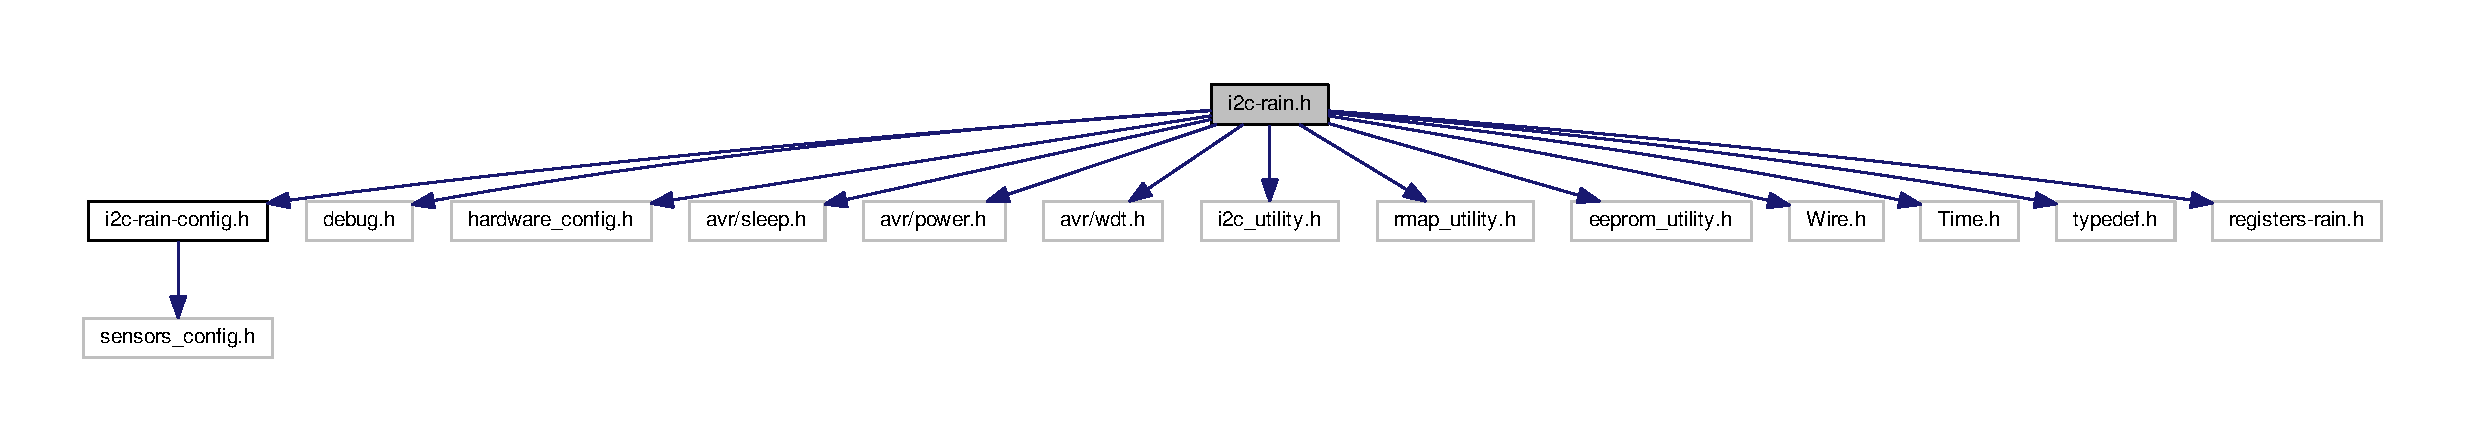
\includegraphics[width=350pt]{i2c-rain_8h__incl}
\end{center}
\end{figure}
This graph shows which files directly or indirectly include this file\+:
\nopagebreak
\begin{figure}[H]
\begin{center}
\leavevmode
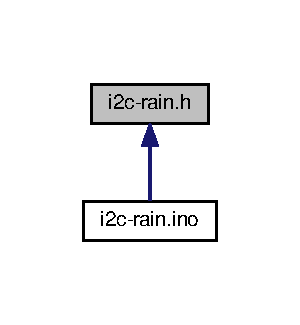
\includegraphics[width=187pt]{i2c-rain_8h__dep__incl}
\end{center}
\end{figure}
\subsection*{Classes}
\begin{DoxyCompactItemize}
\item 
struct \hyperlink{structconfiguration__t}{configuration\+\_\+t}
\begin{DoxyCompactList}\small\item\em E\+E\+P\+R\+OM saved configuration. \end{DoxyCompactList}\item 
struct \hyperlink{structreadable__data__t}{readable\+\_\+data\+\_\+t}
\begin{DoxyCompactList}\small\item\em Readable data through i2c bus. \end{DoxyCompactList}\item 
struct \hyperlink{structwritable__data__t}{writable\+\_\+data\+\_\+t}
\begin{DoxyCompactList}\small\item\em Writable data through i2c bus. \end{DoxyCompactList}\end{DoxyCompactItemize}
\subsection*{Enumerations}
\begin{DoxyCompactItemize}
\item 
enum \hyperlink{i2c-rain_8h_aa0aafed44fec19806d8f9ad834be1248}{state\+\_\+t} \{ \newline
\hyperlink{i2c-rain_8h_aa0aafed44fec19806d8f9ad834be1248a0cb1b2c6a7db1f1084886c98909a3f36}{I\+N\+IT}, 
\hyperlink{i2c-rain_8h_aa0aafed44fec19806d8f9ad834be1248a34f1df650a5075369a6827770c433a91}{T\+A\+S\+K\+S\+\_\+\+E\+X\+E\+C\+U\+T\+I\+ON}, 
\hyperlink{i2c-rain_8h_aa0aafed44fec19806d8f9ad834be1248adc6f24fd6915a3f2786a1b7045406924}{E\+ND}, 
\hyperlink{i2c-th_8h_aa0aafed44fec19806d8f9ad834be1248a0cb1b2c6a7db1f1084886c98909a3f36}{I\+N\+IT}, 
\newline
\hyperlink{i2c-th_8h_aa0aafed44fec19806d8f9ad834be1248a34f1df650a5075369a6827770c433a91}{T\+A\+S\+K\+S\+\_\+\+E\+X\+E\+C\+U\+T\+I\+ON}, 
\hyperlink{i2c-th_8h_aa0aafed44fec19806d8f9ad834be1248adc6f24fd6915a3f2786a1b7045406924}{E\+ND}, 
\hyperlink{rmap_8h_aa0aafed44fec19806d8f9ad834be1248a0cb1b2c6a7db1f1084886c98909a3f36}{I\+N\+IT}, 
\hyperlink{rmap_8h_aa0aafed44fec19806d8f9ad834be1248a34f1df650a5075369a6827770c433a91}{T\+A\+S\+K\+S\+\_\+\+E\+X\+E\+C\+U\+T\+I\+ON}, 
\newline
\hyperlink{rmap_8h_aa0aafed44fec19806d8f9ad834be1248adc6f24fd6915a3f2786a1b7045406924}{E\+ND}
 \}\begin{DoxyCompactList}\small\item\em Main loop finite state machine. \end{DoxyCompactList}
\item 
enum \hyperlink{i2c-rain_8h_a7935f2f599e6a870190d4ae0a86205ba}{tipping\+\_\+bucket\+\_\+state\+\_\+t} \{ \hyperlink{i2c-rain_8h_a7935f2f599e6a870190d4ae0a86205baa0b7c7807059f943bc642578373d65287}{T\+I\+P\+P\+I\+N\+G\+\_\+\+B\+U\+C\+K\+E\+T\+\_\+\+I\+N\+IT}, 
\hyperlink{i2c-rain_8h_a7935f2f599e6a870190d4ae0a86205baa292adccffc71f51ae82f4e219a03e341}{T\+I\+P\+P\+I\+N\+G\+\_\+\+B\+U\+C\+K\+E\+T\+\_\+\+R\+E\+AD}, 
\hyperlink{i2c-rain_8h_a7935f2f599e6a870190d4ae0a86205baa27bb1d47c1289d872321404357c8d2e7}{T\+I\+P\+P\+I\+N\+G\+\_\+\+B\+U\+C\+K\+E\+T\+\_\+\+E\+ND}, 
\hyperlink{i2c-rain_8h_a7935f2f599e6a870190d4ae0a86205baa563187c281a3c4faf3684472339c78c1}{T\+I\+P\+P\+I\+N\+G\+\_\+\+B\+U\+C\+K\+E\+T\+\_\+\+W\+A\+I\+T\+\_\+\+S\+T\+A\+TE}
 \}\begin{DoxyCompactList}\small\item\em Tipping bucket task finite state machine. \end{DoxyCompactList}
\end{DoxyCompactItemize}
\subsection*{Functions}
\begin{DoxyCompactItemize}
\item 
void \hyperlink{i2c-rain_8h_afb98a0f07c30784284f48271ffe02b97}{init\+\_\+power\+\_\+down} (uint32\+\_\+t $\ast$time\+\_\+ms, uint32\+\_\+t debouncing\+\_\+ms)
\begin{DoxyCompactList}\small\item\em Enter power down mode. \end{DoxyCompactList}\item 
void \hyperlink{i2c-rain_8h_a980e73df66b14b1190bc25da430a4f12}{init\+\_\+wdt} (uint8\+\_\+t wdt\+\_\+timer)
\begin{DoxyCompactList}\small\item\em Init watchdog. \end{DoxyCompactList}\item 
void \hyperlink{i2c-rain_8h_a348d23d5899ce59d18975284dfb0afc0}{init\+\_\+system} (void)
\begin{DoxyCompactList}\small\item\em Init system. \end{DoxyCompactList}\item 
void \hyperlink{i2c-rain_8h_ad438327c9cf783bd9c519ce8b8ef3bfa}{init\+\_\+buffers} (void)
\begin{DoxyCompactList}\small\item\em Init buffers. \end{DoxyCompactList}\item 
void \hyperlink{i2c-rain_8h_a2aae2290a141fddcea3fb6009acbb445}{init\+\_\+tasks} (void)
\begin{DoxyCompactList}\small\item\em Init tasks variable and state. \end{DoxyCompactList}\item 
void \hyperlink{i2c-rain_8h_aa9c113540346b54d49b2a596e6ba8480}{init\+\_\+pins} (void)
\begin{DoxyCompactList}\small\item\em Init hardware pins. \end{DoxyCompactList}\item 
void \hyperlink{i2c-rain_8h_a7c21452937863fa02a29654247eef09b}{init\+\_\+wire} (void)
\begin{DoxyCompactList}\small\item\em Init wire (i2c) library and performs checks on the bus. \end{DoxyCompactList}\item 
void \hyperlink{i2c-rain_8h_a4454f968b2402a0e61deb15ab2571dab}{init\+\_\+spi} (void)
\begin{DoxyCompactList}\small\item\em Init S\+PI library. \end{DoxyCompactList}\item 
void \hyperlink{i2c-rain_8h_a88533ad02465ce52d4e6de7b2095ec32}{init\+\_\+rtc} (void)
\begin{DoxyCompactList}\small\item\em Init R\+TC module. \end{DoxyCompactList}\item 
void \hyperlink{i2c-rain_8h_ad7577ba7f06f417a019b69da8682ede5}{init\+\_\+sensors} (void)
\begin{DoxyCompactList}\small\item\em Create and setup sensors. \end{DoxyCompactList}\item 
void \hyperlink{i2c-rain_8h_ab08b9047f47849f399950705e769be2e}{print\+\_\+configuration} (void)
\begin{DoxyCompactList}\small\item\em Print current configuration. \end{DoxyCompactList}\item 
void \hyperlink{i2c-rain_8h_a1be652e7d942160a14a560e0be837358}{load\+\_\+configuration} (void)
\begin{DoxyCompactList}\small\item\em Load configuration from E\+E\+P\+R\+OM. \end{DoxyCompactList}\item 
void \hyperlink{i2c-rain_8h_a8801fa7c9f323c5b8b9b2bb5b1c438ff}{save\+\_\+configuration} (bool)
\begin{DoxyCompactList}\small\item\em Save configuration to E\+E\+P\+R\+OM. \end{DoxyCompactList}\item 
void \hyperlink{i2c-rain_8h_aaad2f6556489c51f2c24302e2cb4188a}{commands} (void)
\begin{DoxyCompactList}\small\item\em Performs specific operations based on the received command. \end{DoxyCompactList}\item 
void \hyperlink{i2c-rain_8h_a717429168fb5542a7b36a94712f7c67e}{reset\+\_\+buffers} (void)
\begin{DoxyCompactList}\small\item\em Reset buffers to default value. \end{DoxyCompactList}\item 
void \hyperlink{i2c-rain_8h_aafa3d59a1bde3085849eee08f110612f}{exchange\+\_\+buffers} (void)
\begin{DoxyCompactList}\small\item\em Exchange reader and writer pointer to buffer. \end{DoxyCompactList}\item 
void \hyperlink{i2c-rain_8h_a8fcd3e091d63c9caff82b8bc3398c279}{tipping\+\_\+bucket\+\_\+task} (void)
\begin{DoxyCompactList}\small\item\em Tipping bucket task. \end{DoxyCompactList}\item 
void \hyperlink{i2c-rain_8h_a9f32a4169471a435e9364460d7b1761d}{command\+\_\+task} (void)
\begin{DoxyCompactList}\small\item\em Execute the command received on i2c bus by reading i2c received data buffer. \end{DoxyCompactList}\item 
void \hyperlink{i2c-rain_8h_ac1da31566bf05976ecb87372278a1ea8}{i2c\+\_\+request\+\_\+interrupt\+\_\+handler} (void)
\begin{DoxyCompactList}\small\item\em I2C request interrupt handler. \end{DoxyCompactList}\item 
void \hyperlink{i2c-rain_8h_a6e27532df66f6bf186654355def5c9af}{i2c\+\_\+receive\+\_\+interrupt\+\_\+handler} (int rx\+\_\+data\+\_\+length)
\begin{DoxyCompactList}\small\item\em I2C receive interrupt handler. \end{DoxyCompactList}\item 
void \hyperlink{i2c-rain_8h_a7fcfeb4fd75663ddccc79030c37d68b9}{tipping\+\_\+bucket\+\_\+interrupt\+\_\+handler} (void)
\begin{DoxyCompactList}\small\item\em Tipping bucket interrupt handler. \end{DoxyCompactList}\end{DoxyCompactItemize}
\subsection*{Variables}
\begin{DoxyCompactItemize}
\item 
\mbox{\Hypertarget{i2c-rain_8h_a32c97d3f8cd6089ccf54e7c423020b7a}\label{i2c-rain_8h_a32c97d3f8cd6089ccf54e7c423020b7a}} 
\hyperlink{structconfiguration__t}{configuration\+\_\+t} \hyperlink{i2c-rain_8h_a32c97d3f8cd6089ccf54e7c423020b7a}{configuration}
\begin{DoxyCompactList}\small\item\em Configuration data. \end{DoxyCompactList}\item 
\mbox{\Hypertarget{i2c-rain_8h_ab7c4666cc43ac73859ace91030494dba}\label{i2c-rain_8h_ab7c4666cc43ac73859ace91030494dba}} 
volatile \hyperlink{structreadable__data__t}{readable\+\_\+data\+\_\+t} \hyperlink{i2c-rain_8h_ab7c4666cc43ac73859ace91030494dba}{readable\+\_\+data\+\_\+1}
\begin{DoxyCompactList}\small\item\em First readable i2c register. \end{DoxyCompactList}\item 
\mbox{\Hypertarget{i2c-rain_8h_af1fd929e13557159958a5328deefd8a3}\label{i2c-rain_8h_af1fd929e13557159958a5328deefd8a3}} 
volatile \hyperlink{structreadable__data__t}{readable\+\_\+data\+\_\+t} \hyperlink{i2c-rain_8h_af1fd929e13557159958a5328deefd8a3}{readable\+\_\+data\+\_\+2}
\begin{DoxyCompactList}\small\item\em Second readable i2c register. \end{DoxyCompactList}\item 
\mbox{\Hypertarget{i2c-rain_8h_af0914001a8977841586be8312dee3656}\label{i2c-rain_8h_af0914001a8977841586be8312dee3656}} 
volatile \hyperlink{structreadable__data__t}{readable\+\_\+data\+\_\+t} $\ast$ \hyperlink{i2c-rain_8h_af0914001a8977841586be8312dee3656}{readable\+\_\+data\+\_\+read\+\_\+ptr}
\begin{DoxyCompactList}\small\item\em Pointer for read data in i2c readable register. \end{DoxyCompactList}\item 
\mbox{\Hypertarget{i2c-rain_8h_ab7eec4069b1ac3d682d74b37921e2707}\label{i2c-rain_8h_ab7eec4069b1ac3d682d74b37921e2707}} 
volatile \hyperlink{structreadable__data__t}{readable\+\_\+data\+\_\+t} $\ast$ \hyperlink{i2c-rain_8h_ab7eec4069b1ac3d682d74b37921e2707}{readable\+\_\+data\+\_\+write\+\_\+ptr}
\begin{DoxyCompactList}\small\item\em Pointer for write data in i2c readable register. \end{DoxyCompactList}\item 
\mbox{\Hypertarget{i2c-rain_8h_ae8dc647e7272fabb6881c64f98b47a01}\label{i2c-rain_8h_ae8dc647e7272fabb6881c64f98b47a01}} 
volatile \hyperlink{structreadable__data__t}{readable\+\_\+data\+\_\+t} $\ast$ \hyperlink{i2c-rain_8h_ae8dc647e7272fabb6881c64f98b47a01}{readable\+\_\+data\+\_\+temp\+\_\+ptr}
\begin{DoxyCompactList}\small\item\em Temporary pointer for exchange read and write pointer for i2c readable register. \end{DoxyCompactList}\item 
\mbox{\Hypertarget{i2c-rain_8h_a4ebae70bf7be3eb353c52c5b4104fca9}\label{i2c-rain_8h_a4ebae70bf7be3eb353c52c5b4104fca9}} 
\hyperlink{structwritable__data__t}{writable\+\_\+data\+\_\+t} \hyperlink{i2c-rain_8h_a4ebae70bf7be3eb353c52c5b4104fca9}{writable\+\_\+data}
\begin{DoxyCompactList}\small\item\em Writable i2c register. \end{DoxyCompactList}\item 
\mbox{\Hypertarget{i2c-rain_8h_a69435b30022db229f79c9a67574008ec}\label{i2c-rain_8h_a69435b30022db229f79c9a67574008ec}} 
\hyperlink{structwritable__data__t}{writable\+\_\+data\+\_\+t} $\ast$ \hyperlink{i2c-rain_8h_a69435b30022db229f79c9a67574008ec}{writable\+\_\+data\+\_\+ptr}
\begin{DoxyCompactList}\small\item\em Pointer for read and write data in i2c writable register. \end{DoxyCompactList}\item 
\mbox{\Hypertarget{i2c-rain_8h_ae75498e0d428e94dd8895abec0af11ca}\label{i2c-rain_8h_ae75498e0d428e94dd8895abec0af11ca}} 
volatile uint8\+\_\+t \hyperlink{i2c-rain_8h_ae75498e0d428e94dd8895abec0af11ca}{readable\+\_\+data\+\_\+address}
\begin{DoxyCompactList}\small\item\em Address of readable i2c register. \end{DoxyCompactList}\item 
\mbox{\Hypertarget{i2c-rain_8h_a202892f30149022049fb90b5db0ddbfa}\label{i2c-rain_8h_a202892f30149022049fb90b5db0ddbfa}} 
volatile uint8\+\_\+t \hyperlink{i2c-rain_8h_a202892f30149022049fb90b5db0ddbfa}{readable\+\_\+data\+\_\+length}
\begin{DoxyCompactList}\small\item\em Number of bytes to read at readable\+\_\+data\+\_\+address. \end{DoxyCompactList}\item 
\mbox{\Hypertarget{i2c-rain_8h_ae22f16db01d254c3709565e8347c05af}\label{i2c-rain_8h_ae22f16db01d254c3709565e8347c05af}} 
volatile uint8\+\_\+t \hyperlink{i2c-rain_8h_ae22f16db01d254c3709565e8347c05af}{i2c\+\_\+rx\+\_\+data} \mbox{[}\hyperlink{hardware__config_8h_aa552d72ce15dd8ca167c4b9323f1f25d}{I2\+C\+\_\+\+M\+A\+X\+\_\+\+D\+A\+T\+A\+\_\+\+L\+E\+N\+G\+TH}\mbox{]}
\begin{DoxyCompactList}\small\item\em Buffer for i2c received data. \end{DoxyCompactList}\item 
\mbox{\Hypertarget{i2c-rain_8h_ad51737114d6776c16525958973815d50}\label{i2c-rain_8h_ad51737114d6776c16525958973815d50}} 
volatile uint8\+\_\+t \hyperlink{i2c-rain_8h_ad51737114d6776c16525958973815d50}{ready\+\_\+tasks\+\_\+count}
\begin{DoxyCompactList}\small\item\em Number of tasks ready to execute. \end{DoxyCompactList}\item 
\mbox{\Hypertarget{i2c-rain_8h_a82dc7d1671e2febacdbd9a3c3a3283cd}\label{i2c-rain_8h_a82dc7d1671e2febacdbd9a3c3a3283cd}} 
uint32\+\_\+t \hyperlink{i2c-rain_8h_a82dc7d1671e2febacdbd9a3c3a3283cd}{awakened\+\_\+event\+\_\+occurred\+\_\+time\+\_\+ms}
\begin{DoxyCompactList}\small\item\em System time (in millisecond) when the system has awakened from power down. \end{DoxyCompactList}\item 
\mbox{\Hypertarget{i2c-rain_8h_a2a9792771d5af0df80ed2adf7c5dc0cf}\label{i2c-rain_8h_a2a9792771d5af0df80ed2adf7c5dc0cf}} 
bool \hyperlink{i2c-rain_8h_a2a9792771d5af0df80ed2adf7c5dc0cf}{is\+\_\+start}
\begin{DoxyCompactList}\small\item\em Execute start command. \end{DoxyCompactList}\item 
\mbox{\Hypertarget{i2c-rain_8h_ad2dc9b34342f31d98c692c9b5ff3c5a9}\label{i2c-rain_8h_ad2dc9b34342f31d98c692c9b5ff3c5a9}} 
bool \hyperlink{i2c-rain_8h_ad2dc9b34342f31d98c692c9b5ff3c5a9}{is\+\_\+stop}
\begin{DoxyCompactList}\small\item\em Execute stop command. \end{DoxyCompactList}\item 
\mbox{\Hypertarget{i2c-rain_8h_a6090a983e62d9556906716dd85f78d9d}\label{i2c-rain_8h_a6090a983e62d9556906716dd85f78d9d}} 
bool \hyperlink{i2c-rain_8h_a6090a983e62d9556906716dd85f78d9d}{is\+\_\+oneshot}
\begin{DoxyCompactList}\small\item\em Received command is in oneshot mode. \end{DoxyCompactList}\item 
\mbox{\Hypertarget{i2c-rain_8h_a75ef189b6b17aa09010c574ed6b01fc3}\label{i2c-rain_8h_a75ef189b6b17aa09010c574ed6b01fc3}} 
bool \hyperlink{i2c-rain_8h_a75ef189b6b17aa09010c574ed6b01fc3}{is\+\_\+continuous}
\begin{DoxyCompactList}\small\item\em Received command is in continuous mode. \end{DoxyCompactList}\item 
\mbox{\Hypertarget{i2c-rain_8h_aa0097a28d3e4da7c88e72228e9b236d2}\label{i2c-rain_8h_aa0097a28d3e4da7c88e72228e9b236d2}} 
volatile uint32\+\_\+t \hyperlink{i2c-rain_8h_aa0097a28d3e4da7c88e72228e9b236d2}{rain\+\_\+tips\+\_\+event\+\_\+occurred\+\_\+time\+\_\+ms}
\begin{DoxyCompactList}\small\item\em System time (in millisecond) when rain tips occured. \end{DoxyCompactList}\item 
\mbox{\Hypertarget{i2c-rain_8h_a5688d7d07e5d53ec6ccd7acce49a728c}\label{i2c-rain_8h_a5688d7d07e5d53ec6ccd7acce49a728c}} 
\hyperlink{structrain__t}{rain\+\_\+t} \hyperlink{i2c-rain_8h_a5688d7d07e5d53ec6ccd7acce49a728c}{rain}
\begin{DoxyCompactList}\small\item\em Rain data. \end{DoxyCompactList}\item 
\mbox{\Hypertarget{i2c-rain_8h_adc6e5733fc3c22f0a7b2914188c49c90}\label{i2c-rain_8h_adc6e5733fc3c22f0a7b2914188c49c90}} 
\hyperlink{i2c-rain_8h_aa0aafed44fec19806d8f9ad834be1248}{state\+\_\+t} \hyperlink{i2c-rain_8h_adc6e5733fc3c22f0a7b2914188c49c90}{state}
\begin{DoxyCompactList}\small\item\em Current main loop state. \end{DoxyCompactList}\item 
\mbox{\Hypertarget{i2c-rain_8h_ad17df11ab3931697018251d1e0e49d4a}\label{i2c-rain_8h_ad17df11ab3931697018251d1e0e49d4a}} 
\hyperlink{i2c-rain_8h_a7935f2f599e6a870190d4ae0a86205ba}{tipping\+\_\+bucket\+\_\+state\+\_\+t} \hyperlink{i2c-rain_8h_ad17df11ab3931697018251d1e0e49d4a}{tipping\+\_\+bucket\+\_\+state}
\begin{DoxyCompactList}\small\item\em Current tipping bucket task state. \end{DoxyCompactList}\item 
\mbox{\Hypertarget{i2c-rain_8h_a28d699d6f58eb0ef202537500dfbd464}\label{i2c-rain_8h_a28d699d6f58eb0ef202537500dfbd464}} 
volatile bool \hyperlink{i2c-rain_8h_a28d699d6f58eb0ef202537500dfbd464}{is\+\_\+event\+\_\+tipping\+\_\+bucket}
\begin{DoxyCompactList}\small\item\em Enable or disable the Tipping Bucket task. \end{DoxyCompactList}\item 
\mbox{\Hypertarget{i2c-rain_8h_a12ae2319a01786793345e264f29368a4}\label{i2c-rain_8h_a12ae2319a01786793345e264f29368a4}} 
volatile bool \hyperlink{i2c-rain_8h_a12ae2319a01786793345e264f29368a4}{is\+\_\+event\+\_\+command\+\_\+task}
\begin{DoxyCompactList}\small\item\em Enable or disable the Command task. \end{DoxyCompactList}\end{DoxyCompactItemize}


\subsection{Enumeration Type Documentation}
\mbox{\Hypertarget{i2c-rain_8h_aa0aafed44fec19806d8f9ad834be1248}\label{i2c-rain_8h_aa0aafed44fec19806d8f9ad834be1248}} 
\index{i2c-\/rain.\+h@{i2c-\/rain.\+h}!state\+\_\+t@{state\+\_\+t}}
\index{state\+\_\+t@{state\+\_\+t}!i2c-\/rain.\+h@{i2c-\/rain.\+h}}
\subsubsection{\texorpdfstring{state\+\_\+t}{state\_t}}
{\footnotesize\ttfamily enum \hyperlink{i2c-rain_8h_aa0aafed44fec19806d8f9ad834be1248}{state\+\_\+t}}



Main loop finite state machine. 

\begin{DoxyEnumFields}{Enumerator}
\raisebox{\heightof{T}}[0pt][0pt]{\index{I\+N\+IT@{I\+N\+IT}!i2c-\/rain.\+h@{i2c-\/rain.\+h}}\index{i2c-\/rain.\+h@{i2c-\/rain.\+h}!I\+N\+IT@{I\+N\+IT}}}\mbox{\Hypertarget{i2c-rain_8h_aa0aafed44fec19806d8f9ad834be1248a0cb1b2c6a7db1f1084886c98909a3f36}\label{i2c-rain_8h_aa0aafed44fec19806d8f9ad834be1248a0cb1b2c6a7db1f1084886c98909a3f36}} 
I\+N\+IT&init tasks and sensors \\
\hline

\raisebox{\heightof{T}}[0pt][0pt]{\index{T\+A\+S\+K\+S\+\_\+\+E\+X\+E\+C\+U\+T\+I\+ON@{T\+A\+S\+K\+S\+\_\+\+E\+X\+E\+C\+U\+T\+I\+ON}!i2c-\/rain.\+h@{i2c-\/rain.\+h}}\index{i2c-\/rain.\+h@{i2c-\/rain.\+h}!T\+A\+S\+K\+S\+\_\+\+E\+X\+E\+C\+U\+T\+I\+ON@{T\+A\+S\+K\+S\+\_\+\+E\+X\+E\+C\+U\+T\+I\+ON}}}\mbox{\Hypertarget{i2c-rain_8h_aa0aafed44fec19806d8f9ad834be1248a34f1df650a5075369a6827770c433a91}\label{i2c-rain_8h_aa0aafed44fec19806d8f9ad834be1248a34f1df650a5075369a6827770c433a91}} 
T\+A\+S\+K\+S\+\_\+\+E\+X\+E\+C\+U\+T\+I\+ON&execute active tasks \\
\hline

\raisebox{\heightof{T}}[0pt][0pt]{\index{E\+ND@{E\+ND}!i2c-\/rain.\+h@{i2c-\/rain.\+h}}\index{i2c-\/rain.\+h@{i2c-\/rain.\+h}!E\+ND@{E\+ND}}}\mbox{\Hypertarget{i2c-rain_8h_aa0aafed44fec19806d8f9ad834be1248adc6f24fd6915a3f2786a1b7045406924}\label{i2c-rain_8h_aa0aafed44fec19806d8f9ad834be1248adc6f24fd6915a3f2786a1b7045406924}} 
E\+ND&go to E\+N\+T\+E\+R\+\_\+\+P\+O\+W\+E\+R\+\_\+\+D\+O\+WN or T\+A\+S\+K\+S\+\_\+\+E\+X\+E\+C\+U\+T\+I\+ON \\
\hline

\raisebox{\heightof{T}}[0pt][0pt]{\index{I\+N\+IT@{I\+N\+IT}!i2c-\/rain.\+h@{i2c-\/rain.\+h}}\index{i2c-\/rain.\+h@{i2c-\/rain.\+h}!I\+N\+IT@{I\+N\+IT}}}\mbox{\Hypertarget{i2c-rain_8h_aa0aafed44fec19806d8f9ad834be1248a0cb1b2c6a7db1f1084886c98909a3f36}\label{i2c-rain_8h_aa0aafed44fec19806d8f9ad834be1248a0cb1b2c6a7db1f1084886c98909a3f36}} 
I\+N\+IT&init tasks and sensors \\
\hline

\raisebox{\heightof{T}}[0pt][0pt]{\index{T\+A\+S\+K\+S\+\_\+\+E\+X\+E\+C\+U\+T\+I\+ON@{T\+A\+S\+K\+S\+\_\+\+E\+X\+E\+C\+U\+T\+I\+ON}!i2c-\/rain.\+h@{i2c-\/rain.\+h}}\index{i2c-\/rain.\+h@{i2c-\/rain.\+h}!T\+A\+S\+K\+S\+\_\+\+E\+X\+E\+C\+U\+T\+I\+ON@{T\+A\+S\+K\+S\+\_\+\+E\+X\+E\+C\+U\+T\+I\+ON}}}\mbox{\Hypertarget{i2c-rain_8h_aa0aafed44fec19806d8f9ad834be1248a34f1df650a5075369a6827770c433a91}\label{i2c-rain_8h_aa0aafed44fec19806d8f9ad834be1248a34f1df650a5075369a6827770c433a91}} 
T\+A\+S\+K\+S\+\_\+\+E\+X\+E\+C\+U\+T\+I\+ON&execute active tasks \\
\hline

\raisebox{\heightof{T}}[0pt][0pt]{\index{E\+ND@{E\+ND}!i2c-\/rain.\+h@{i2c-\/rain.\+h}}\index{i2c-\/rain.\+h@{i2c-\/rain.\+h}!E\+ND@{E\+ND}}}\mbox{\Hypertarget{i2c-rain_8h_aa0aafed44fec19806d8f9ad834be1248adc6f24fd6915a3f2786a1b7045406924}\label{i2c-rain_8h_aa0aafed44fec19806d8f9ad834be1248adc6f24fd6915a3f2786a1b7045406924}} 
E\+ND&go to E\+N\+T\+E\+R\+\_\+\+P\+O\+W\+E\+R\+\_\+\+D\+O\+WN or T\+A\+S\+K\+S\+\_\+\+E\+X\+E\+C\+U\+T\+I\+ON \\
\hline

\raisebox{\heightof{T}}[0pt][0pt]{\index{I\+N\+IT@{I\+N\+IT}!i2c-\/rain.\+h@{i2c-\/rain.\+h}}\index{i2c-\/rain.\+h@{i2c-\/rain.\+h}!I\+N\+IT@{I\+N\+IT}}}\mbox{\Hypertarget{i2c-rain_8h_aa0aafed44fec19806d8f9ad834be1248a0cb1b2c6a7db1f1084886c98909a3f36}\label{i2c-rain_8h_aa0aafed44fec19806d8f9ad834be1248a0cb1b2c6a7db1f1084886c98909a3f36}} 
I\+N\+IT&init tasks and sensors \\
\hline

\raisebox{\heightof{T}}[0pt][0pt]{\index{T\+A\+S\+K\+S\+\_\+\+E\+X\+E\+C\+U\+T\+I\+ON@{T\+A\+S\+K\+S\+\_\+\+E\+X\+E\+C\+U\+T\+I\+ON}!i2c-\/rain.\+h@{i2c-\/rain.\+h}}\index{i2c-\/rain.\+h@{i2c-\/rain.\+h}!T\+A\+S\+K\+S\+\_\+\+E\+X\+E\+C\+U\+T\+I\+ON@{T\+A\+S\+K\+S\+\_\+\+E\+X\+E\+C\+U\+T\+I\+ON}}}\mbox{\Hypertarget{i2c-rain_8h_aa0aafed44fec19806d8f9ad834be1248a34f1df650a5075369a6827770c433a91}\label{i2c-rain_8h_aa0aafed44fec19806d8f9ad834be1248a34f1df650a5075369a6827770c433a91}} 
T\+A\+S\+K\+S\+\_\+\+E\+X\+E\+C\+U\+T\+I\+ON&execute active tasks \\
\hline

\raisebox{\heightof{T}}[0pt][0pt]{\index{E\+ND@{E\+ND}!i2c-\/rain.\+h@{i2c-\/rain.\+h}}\index{i2c-\/rain.\+h@{i2c-\/rain.\+h}!E\+ND@{E\+ND}}}\mbox{\Hypertarget{i2c-rain_8h_aa0aafed44fec19806d8f9ad834be1248adc6f24fd6915a3f2786a1b7045406924}\label{i2c-rain_8h_aa0aafed44fec19806d8f9ad834be1248adc6f24fd6915a3f2786a1b7045406924}} 
E\+ND&go to E\+N\+T\+E\+R\+\_\+\+P\+O\+W\+E\+R\+\_\+\+D\+O\+WN or T\+A\+S\+K\+S\+\_\+\+E\+X\+E\+C\+U\+T\+I\+ON \\
\hline

\end{DoxyEnumFields}
\mbox{\Hypertarget{i2c-rain_8h_a7935f2f599e6a870190d4ae0a86205ba}\label{i2c-rain_8h_a7935f2f599e6a870190d4ae0a86205ba}} 
\index{i2c-\/rain.\+h@{i2c-\/rain.\+h}!tipping\+\_\+bucket\+\_\+state\+\_\+t@{tipping\+\_\+bucket\+\_\+state\+\_\+t}}
\index{tipping\+\_\+bucket\+\_\+state\+\_\+t@{tipping\+\_\+bucket\+\_\+state\+\_\+t}!i2c-\/rain.\+h@{i2c-\/rain.\+h}}
\subsubsection{\texorpdfstring{tipping\+\_\+bucket\+\_\+state\+\_\+t}{tipping\_bucket\_state\_t}}
{\footnotesize\ttfamily enum \hyperlink{i2c-rain_8h_a7935f2f599e6a870190d4ae0a86205ba}{tipping\+\_\+bucket\+\_\+state\+\_\+t}}



Tipping bucket task finite state machine. 

\begin{DoxyEnumFields}{Enumerator}
\raisebox{\heightof{T}}[0pt][0pt]{\index{T\+I\+P\+P\+I\+N\+G\+\_\+\+B\+U\+C\+K\+E\+T\+\_\+\+I\+N\+IT@{T\+I\+P\+P\+I\+N\+G\+\_\+\+B\+U\+C\+K\+E\+T\+\_\+\+I\+N\+IT}!i2c-\/rain.\+h@{i2c-\/rain.\+h}}\index{i2c-\/rain.\+h@{i2c-\/rain.\+h}!T\+I\+P\+P\+I\+N\+G\+\_\+\+B\+U\+C\+K\+E\+T\+\_\+\+I\+N\+IT@{T\+I\+P\+P\+I\+N\+G\+\_\+\+B\+U\+C\+K\+E\+T\+\_\+\+I\+N\+IT}}}\mbox{\Hypertarget{i2c-rain_8h_a7935f2f599e6a870190d4ae0a86205baa0b7c7807059f943bc642578373d65287}\label{i2c-rain_8h_a7935f2f599e6a870190d4ae0a86205baa0b7c7807059f943bc642578373d65287}} 
T\+I\+P\+P\+I\+N\+G\+\_\+\+B\+U\+C\+K\+E\+T\+\_\+\+I\+N\+IT&init task variables \\
\hline

\raisebox{\heightof{T}}[0pt][0pt]{\index{T\+I\+P\+P\+I\+N\+G\+\_\+\+B\+U\+C\+K\+E\+T\+\_\+\+R\+E\+AD@{T\+I\+P\+P\+I\+N\+G\+\_\+\+B\+U\+C\+K\+E\+T\+\_\+\+R\+E\+AD}!i2c-\/rain.\+h@{i2c-\/rain.\+h}}\index{i2c-\/rain.\+h@{i2c-\/rain.\+h}!T\+I\+P\+P\+I\+N\+G\+\_\+\+B\+U\+C\+K\+E\+T\+\_\+\+R\+E\+AD@{T\+I\+P\+P\+I\+N\+G\+\_\+\+B\+U\+C\+K\+E\+T\+\_\+\+R\+E\+AD}}}\mbox{\Hypertarget{i2c-rain_8h_a7935f2f599e6a870190d4ae0a86205baa292adccffc71f51ae82f4e219a03e341}\label{i2c-rain_8h_a7935f2f599e6a870190d4ae0a86205baa292adccffc71f51ae82f4e219a03e341}} 
T\+I\+P\+P\+I\+N\+G\+\_\+\+B\+U\+C\+K\+E\+T\+\_\+\+R\+E\+AD&read rain tips from variable shared with tipping bucket interrupt \\
\hline

\raisebox{\heightof{T}}[0pt][0pt]{\index{T\+I\+P\+P\+I\+N\+G\+\_\+\+B\+U\+C\+K\+E\+T\+\_\+\+E\+ND@{T\+I\+P\+P\+I\+N\+G\+\_\+\+B\+U\+C\+K\+E\+T\+\_\+\+E\+ND}!i2c-\/rain.\+h@{i2c-\/rain.\+h}}\index{i2c-\/rain.\+h@{i2c-\/rain.\+h}!T\+I\+P\+P\+I\+N\+G\+\_\+\+B\+U\+C\+K\+E\+T\+\_\+\+E\+ND@{T\+I\+P\+P\+I\+N\+G\+\_\+\+B\+U\+C\+K\+E\+T\+\_\+\+E\+ND}}}\mbox{\Hypertarget{i2c-rain_8h_a7935f2f599e6a870190d4ae0a86205baa27bb1d47c1289d872321404357c8d2e7}\label{i2c-rain_8h_a7935f2f599e6a870190d4ae0a86205baa27bb1d47c1289d872321404357c8d2e7}} 
T\+I\+P\+P\+I\+N\+G\+\_\+\+B\+U\+C\+K\+E\+T\+\_\+\+E\+ND&performs end operations and deactivate task \\
\hline

\raisebox{\heightof{T}}[0pt][0pt]{\index{T\+I\+P\+P\+I\+N\+G\+\_\+\+B\+U\+C\+K\+E\+T\+\_\+\+W\+A\+I\+T\+\_\+\+S\+T\+A\+TE@{T\+I\+P\+P\+I\+N\+G\+\_\+\+B\+U\+C\+K\+E\+T\+\_\+\+W\+A\+I\+T\+\_\+\+S\+T\+A\+TE}!i2c-\/rain.\+h@{i2c-\/rain.\+h}}\index{i2c-\/rain.\+h@{i2c-\/rain.\+h}!T\+I\+P\+P\+I\+N\+G\+\_\+\+B\+U\+C\+K\+E\+T\+\_\+\+W\+A\+I\+T\+\_\+\+S\+T\+A\+TE@{T\+I\+P\+P\+I\+N\+G\+\_\+\+B\+U\+C\+K\+E\+T\+\_\+\+W\+A\+I\+T\+\_\+\+S\+T\+A\+TE}}}\mbox{\Hypertarget{i2c-rain_8h_a7935f2f599e6a870190d4ae0a86205baa563187c281a3c4faf3684472339c78c1}\label{i2c-rain_8h_a7935f2f599e6a870190d4ae0a86205baa563187c281a3c4faf3684472339c78c1}} 
T\+I\+P\+P\+I\+N\+G\+\_\+\+B\+U\+C\+K\+E\+T\+\_\+\+W\+A\+I\+T\+\_\+\+S\+T\+A\+TE&non-\/blocking waiting time \\
\hline

\end{DoxyEnumFields}


\subsection{Function Documentation}
\mbox{\Hypertarget{i2c-rain_8h_a9f32a4169471a435e9364460d7b1761d}\label{i2c-rain_8h_a9f32a4169471a435e9364460d7b1761d}} 
\index{i2c-\/rain.\+h@{i2c-\/rain.\+h}!command\+\_\+task@{command\+\_\+task}}
\index{command\+\_\+task@{command\+\_\+task}!i2c-\/rain.\+h@{i2c-\/rain.\+h}}
\subsubsection{\texorpdfstring{command\+\_\+task()}{command\_task()}}
{\footnotesize\ttfamily void command\+\_\+task (\begin{DoxyParamCaption}\item[{void}]{ }\end{DoxyParamCaption})}



Execute the command received on i2c bus by reading i2c received data buffer. 

Command Task. Execute the command received on i2c bus by reading i2c received data buffer.

\begin{DoxyReturn}{Returns}
void. 
\end{DoxyReturn}
\mbox{\Hypertarget{i2c-rain_8h_aaad2f6556489c51f2c24302e2cb4188a}\label{i2c-rain_8h_aaad2f6556489c51f2c24302e2cb4188a}} 
\index{i2c-\/rain.\+h@{i2c-\/rain.\+h}!commands@{commands}}
\index{commands@{commands}!i2c-\/rain.\+h@{i2c-\/rain.\+h}}
\subsubsection{\texorpdfstring{commands()}{commands()}}
{\footnotesize\ttfamily void commands (\begin{DoxyParamCaption}\item[{void}]{ }\end{DoxyParamCaption})}



Performs specific operations based on the received command. 

\begin{DoxyReturn}{Returns}
void. 
\end{DoxyReturn}
C\+O\+N\+T\+I\+N\+U\+O\+US S\+T\+A\+RT

C\+O\+N\+T\+I\+N\+U\+O\+US S\+T\+OP

C\+O\+N\+T\+I\+N\+U\+O\+US S\+T\+A\+R\+T-\/\+S\+T\+OP

O\+N\+E\+S\+H\+OT S\+T\+A\+RT

O\+N\+E\+S\+H\+OT S\+T\+OP

O\+N\+E\+S\+H\+OT S\+T\+A\+R\+T-\/\+S\+T\+OP \mbox{\Hypertarget{i2c-rain_8h_aafa3d59a1bde3085849eee08f110612f}\label{i2c-rain_8h_aafa3d59a1bde3085849eee08f110612f}} 
\index{i2c-\/rain.\+h@{i2c-\/rain.\+h}!exchange\+\_\+buffers@{exchange\+\_\+buffers}}
\index{exchange\+\_\+buffers@{exchange\+\_\+buffers}!i2c-\/rain.\+h@{i2c-\/rain.\+h}}
\subsubsection{\texorpdfstring{exchange\+\_\+buffers()}{exchange\_buffers()}}
{\footnotesize\ttfamily void exchange\+\_\+buffers (\begin{DoxyParamCaption}\item[{void}]{ }\end{DoxyParamCaption})}



Exchange reader and writer pointer to buffer. 

\begin{DoxyReturn}{Returns}
void. 
\end{DoxyReturn}
\mbox{\Hypertarget{i2c-rain_8h_a6e27532df66f6bf186654355def5c9af}\label{i2c-rain_8h_a6e27532df66f6bf186654355def5c9af}} 
\index{i2c-\/rain.\+h@{i2c-\/rain.\+h}!i2c\+\_\+receive\+\_\+interrupt\+\_\+handler@{i2c\+\_\+receive\+\_\+interrupt\+\_\+handler}}
\index{i2c\+\_\+receive\+\_\+interrupt\+\_\+handler@{i2c\+\_\+receive\+\_\+interrupt\+\_\+handler}!i2c-\/rain.\+h@{i2c-\/rain.\+h}}
\subsubsection{\texorpdfstring{i2c\+\_\+receive\+\_\+interrupt\+\_\+handler()}{i2c\_receive\_interrupt\_handler()}}
{\footnotesize\ttfamily void i2c\+\_\+receive\+\_\+interrupt\+\_\+handler (\begin{DoxyParamCaption}\item[{int}]{rx\+\_\+data\+\_\+length }\end{DoxyParamCaption})}



I2C receive interrupt handler. 


\begin{DoxyParams}[1]{Parameters}
\mbox{\tt in}  & {\em rx\+\_\+data\+\_\+length} & received data length in bytes. \\
\hline
\end{DoxyParams}
\begin{DoxyReturn}{Returns}
void. 
\end{DoxyReturn}
read rx\+\_\+data\+\_\+length bytes of data from i2c bus

it is a registers read?

offset in readable\+\_\+data\+\_\+read\+\_\+ptr buffer

length (in butes) of data to be read in readable\+\_\+data\+\_\+read\+\_\+ptr

it is a command?

enable Command task

it is a registers write? \mbox{\Hypertarget{i2c-rain_8h_ac1da31566bf05976ecb87372278a1ea8}\label{i2c-rain_8h_ac1da31566bf05976ecb87372278a1ea8}} 
\index{i2c-\/rain.\+h@{i2c-\/rain.\+h}!i2c\+\_\+request\+\_\+interrupt\+\_\+handler@{i2c\+\_\+request\+\_\+interrupt\+\_\+handler}}
\index{i2c\+\_\+request\+\_\+interrupt\+\_\+handler@{i2c\+\_\+request\+\_\+interrupt\+\_\+handler}!i2c-\/rain.\+h@{i2c-\/rain.\+h}}
\subsubsection{\texorpdfstring{i2c\+\_\+request\+\_\+interrupt\+\_\+handler()}{i2c\_request\_interrupt\_handler()}}
{\footnotesize\ttfamily void i2c\+\_\+request\+\_\+interrupt\+\_\+handler (\begin{DoxyParamCaption}\item[{void}]{ }\end{DoxyParamCaption})}



I2C request interrupt handler. 

\begin{DoxyReturn}{Returns}
void. 
\end{DoxyReturn}
write readable\+\_\+data\+\_\+length bytes of data stored in readable\+\_\+data\+\_\+read\+\_\+ptr (base) + readable\+\_\+data\+\_\+address (offset) on i2c bus \mbox{\Hypertarget{i2c-rain_8h_ad438327c9cf783bd9c519ce8b8ef3bfa}\label{i2c-rain_8h_ad438327c9cf783bd9c519ce8b8ef3bfa}} 
\index{i2c-\/rain.\+h@{i2c-\/rain.\+h}!init\+\_\+buffers@{init\+\_\+buffers}}
\index{init\+\_\+buffers@{init\+\_\+buffers}!i2c-\/rain.\+h@{i2c-\/rain.\+h}}
\subsubsection{\texorpdfstring{init\+\_\+buffers()}{init\_buffers()}}
{\footnotesize\ttfamily void init\+\_\+buffers (\begin{DoxyParamCaption}\item[{void}]{ }\end{DoxyParamCaption})}



Init buffers. 

\begin{DoxyReturn}{Returns}
void. 
\end{DoxyReturn}
copy readable\+\_\+data\+\_\+2 in readable\+\_\+data\+\_\+1 \mbox{\Hypertarget{i2c-rain_8h_aa9c113540346b54d49b2a596e6ba8480}\label{i2c-rain_8h_aa9c113540346b54d49b2a596e6ba8480}} 
\index{i2c-\/rain.\+h@{i2c-\/rain.\+h}!init\+\_\+pins@{init\+\_\+pins}}
\index{init\+\_\+pins@{init\+\_\+pins}!i2c-\/rain.\+h@{i2c-\/rain.\+h}}
\subsubsection{\texorpdfstring{init\+\_\+pins()}{init\_pins()}}
{\footnotesize\ttfamily void init\+\_\+pins (\begin{DoxyParamCaption}\item[{void}]{ }\end{DoxyParamCaption})}



Init hardware pins. 

\begin{DoxyReturn}{Returns}
void. 
\end{DoxyReturn}
\mbox{\Hypertarget{i2c-rain_8h_afb98a0f07c30784284f48271ffe02b97}\label{i2c-rain_8h_afb98a0f07c30784284f48271ffe02b97}} 
\index{i2c-\/rain.\+h@{i2c-\/rain.\+h}!init\+\_\+power\+\_\+down@{init\+\_\+power\+\_\+down}}
\index{init\+\_\+power\+\_\+down@{init\+\_\+power\+\_\+down}!i2c-\/rain.\+h@{i2c-\/rain.\+h}}
\subsubsection{\texorpdfstring{init\+\_\+power\+\_\+down()}{init\_power\_down()}}
{\footnotesize\ttfamily void init\+\_\+power\+\_\+down (\begin{DoxyParamCaption}\item[{uint32\+\_\+t $\ast$}]{time\+\_\+ms,  }\item[{uint32\+\_\+t}]{debouncing\+\_\+ms }\end{DoxyParamCaption})}



Enter power down mode. 


\begin{DoxyParams}{Parameters}
{\em time\+\_\+ms} & pointer to a variable to save the last instant you entered power down. \\
\hline
{\em debouncing\+\_\+ms} & delay to power down. \\
\hline
\end{DoxyParams}
\begin{DoxyReturn}{Returns}
void. 
\end{DoxyReturn}
turn off brown-\/out \mbox{\Hypertarget{i2c-rain_8h_a88533ad02465ce52d4e6de7b2095ec32}\label{i2c-rain_8h_a88533ad02465ce52d4e6de7b2095ec32}} 
\index{i2c-\/rain.\+h@{i2c-\/rain.\+h}!init\+\_\+rtc@{init\+\_\+rtc}}
\index{init\+\_\+rtc@{init\+\_\+rtc}!i2c-\/rain.\+h@{i2c-\/rain.\+h}}
\subsubsection{\texorpdfstring{init\+\_\+rtc()}{init\_rtc()}}
{\footnotesize\ttfamily void init\+\_\+rtc (\begin{DoxyParamCaption}\item[{void}]{ }\end{DoxyParamCaption})}



Init R\+TC module. 

\begin{DoxyReturn}{Returns}
void. 
\end{DoxyReturn}
\mbox{\Hypertarget{i2c-rain_8h_ad7577ba7f06f417a019b69da8682ede5}\label{i2c-rain_8h_ad7577ba7f06f417a019b69da8682ede5}} 
\index{i2c-\/rain.\+h@{i2c-\/rain.\+h}!init\+\_\+sensors@{init\+\_\+sensors}}
\index{init\+\_\+sensors@{init\+\_\+sensors}!i2c-\/rain.\+h@{i2c-\/rain.\+h}}
\subsubsection{\texorpdfstring{init\+\_\+sensors()}{init\_sensors()}}
{\footnotesize\ttfamily void init\+\_\+sensors (\begin{DoxyParamCaption}\item[{void}]{ }\end{DoxyParamCaption})}



Create and setup sensors. 

\begin{DoxyReturn}{Returns}
void. 
\end{DoxyReturn}
\mbox{\Hypertarget{i2c-rain_8h_a4454f968b2402a0e61deb15ab2571dab}\label{i2c-rain_8h_a4454f968b2402a0e61deb15ab2571dab}} 
\index{i2c-\/rain.\+h@{i2c-\/rain.\+h}!init\+\_\+spi@{init\+\_\+spi}}
\index{init\+\_\+spi@{init\+\_\+spi}!i2c-\/rain.\+h@{i2c-\/rain.\+h}}
\subsubsection{\texorpdfstring{init\+\_\+spi()}{init\_spi()}}
{\footnotesize\ttfamily void init\+\_\+spi (\begin{DoxyParamCaption}\item[{void}]{ }\end{DoxyParamCaption})}



Init S\+PI library. 

\begin{DoxyReturn}{Returns}
void. 
\end{DoxyReturn}
\mbox{\Hypertarget{i2c-rain_8h_a348d23d5899ce59d18975284dfb0afc0}\label{i2c-rain_8h_a348d23d5899ce59d18975284dfb0afc0}} 
\index{i2c-\/rain.\+h@{i2c-\/rain.\+h}!init\+\_\+system@{init\+\_\+system}}
\index{init\+\_\+system@{init\+\_\+system}!i2c-\/rain.\+h@{i2c-\/rain.\+h}}
\subsubsection{\texorpdfstring{init\+\_\+system()}{init\_system()}}
{\footnotesize\ttfamily void init\+\_\+system (\begin{DoxyParamCaption}\item[{void}]{ }\end{DoxyParamCaption})}



Init system. 

\begin{DoxyReturn}{Returns}
void. 
\end{DoxyReturn}
main loop state \mbox{\Hypertarget{i2c-rain_8h_a2aae2290a141fddcea3fb6009acbb445}\label{i2c-rain_8h_a2aae2290a141fddcea3fb6009acbb445}} 
\index{i2c-\/rain.\+h@{i2c-\/rain.\+h}!init\+\_\+tasks@{init\+\_\+tasks}}
\index{init\+\_\+tasks@{init\+\_\+tasks}!i2c-\/rain.\+h@{i2c-\/rain.\+h}}
\subsubsection{\texorpdfstring{init\+\_\+tasks()}{init\_tasks()}}
{\footnotesize\ttfamily void init\+\_\+tasks (\begin{DoxyParamCaption}\item[{void}]{ }\end{DoxyParamCaption})}



Init tasks variable and state. 

\begin{DoxyReturn}{Returns}
void. 
\end{DoxyReturn}
no tasks ready

reset samples\+\_\+count value \mbox{\Hypertarget{i2c-rain_8h_a980e73df66b14b1190bc25da430a4f12}\label{i2c-rain_8h_a980e73df66b14b1190bc25da430a4f12}} 
\index{i2c-\/rain.\+h@{i2c-\/rain.\+h}!init\+\_\+wdt@{init\+\_\+wdt}}
\index{init\+\_\+wdt@{init\+\_\+wdt}!i2c-\/rain.\+h@{i2c-\/rain.\+h}}
\subsubsection{\texorpdfstring{init\+\_\+wdt()}{init\_wdt()}}
{\footnotesize\ttfamily void init\+\_\+wdt (\begin{DoxyParamCaption}\item[{uint8\+\_\+t}]{wdt\+\_\+timer }\end{DoxyParamCaption})}



Init watchdog. 


\begin{DoxyParams}{Parameters}
{\em wdt\+\_\+timer} & a time value for init watchdog (W\+D\+T\+O\+\_\+xxxx). \\
\hline
\end{DoxyParams}
\begin{DoxyReturn}{Returns}
void. 
\end{DoxyReturn}
\mbox{\Hypertarget{i2c-rain_8h_a7c21452937863fa02a29654247eef09b}\label{i2c-rain_8h_a7c21452937863fa02a29654247eef09b}} 
\index{i2c-\/rain.\+h@{i2c-\/rain.\+h}!init\+\_\+wire@{init\+\_\+wire}}
\index{init\+\_\+wire@{init\+\_\+wire}!i2c-\/rain.\+h@{i2c-\/rain.\+h}}
\subsubsection{\texorpdfstring{init\+\_\+wire()}{init\_wire()}}
{\footnotesize\ttfamily void init\+\_\+wire (\begin{DoxyParamCaption}\item[{void}]{ }\end{DoxyParamCaption})}



Init wire (i2c) library and performs checks on the bus. 

\begin{DoxyReturn}{Returns}
void. 
\end{DoxyReturn}
clear the I2C bus first before calling Wire.\+begin()

wait for watchdog reboot \mbox{\Hypertarget{i2c-rain_8h_a1be652e7d942160a14a560e0be837358}\label{i2c-rain_8h_a1be652e7d942160a14a560e0be837358}} 
\index{i2c-\/rain.\+h@{i2c-\/rain.\+h}!load\+\_\+configuration@{load\+\_\+configuration}}
\index{load\+\_\+configuration@{load\+\_\+configuration}!i2c-\/rain.\+h@{i2c-\/rain.\+h}}
\subsubsection{\texorpdfstring{load\+\_\+configuration()}{load\_configuration()}}
{\footnotesize\ttfamily void load\+\_\+configuration (\begin{DoxyParamCaption}\item[{void}]{ }\end{DoxyParamCaption})}



Load configuration from E\+E\+P\+R\+OM. 

\begin{DoxyReturn}{Returns}
void. 
\end{DoxyReturn}
read configuration from eeprom \mbox{\Hypertarget{i2c-rain_8h_ab08b9047f47849f399950705e769be2e}\label{i2c-rain_8h_ab08b9047f47849f399950705e769be2e}} 
\index{i2c-\/rain.\+h@{i2c-\/rain.\+h}!print\+\_\+configuration@{print\+\_\+configuration}}
\index{print\+\_\+configuration@{print\+\_\+configuration}!i2c-\/rain.\+h@{i2c-\/rain.\+h}}
\subsubsection{\texorpdfstring{print\+\_\+configuration()}{print\_configuration()}}
{\footnotesize\ttfamily void print\+\_\+configuration (\begin{DoxyParamCaption}\item[{void}]{ }\end{DoxyParamCaption})}



Print current configuration. 

\begin{DoxyReturn}{Returns}
void. 
\end{DoxyReturn}
\mbox{\Hypertarget{i2c-rain_8h_a717429168fb5542a7b36a94712f7c67e}\label{i2c-rain_8h_a717429168fb5542a7b36a94712f7c67e}} 
\index{i2c-\/rain.\+h@{i2c-\/rain.\+h}!reset\+\_\+buffers@{reset\+\_\+buffers}}
\index{reset\+\_\+buffers@{reset\+\_\+buffers}!i2c-\/rain.\+h@{i2c-\/rain.\+h}}
\subsubsection{\texorpdfstring{reset\+\_\+buffers()}{reset\_buffers()}}
{\footnotesize\ttfamily void reset\+\_\+buffers (\begin{DoxyParamCaption}\item[{void}]{ }\end{DoxyParamCaption})}



Reset buffers to default value. 

\begin{DoxyReturn}{Returns}
void. 
\end{DoxyReturn}
\mbox{\Hypertarget{i2c-rain_8h_a8801fa7c9f323c5b8b9b2bb5b1c438ff}\label{i2c-rain_8h_a8801fa7c9f323c5b8b9b2bb5b1c438ff}} 
\index{i2c-\/rain.\+h@{i2c-\/rain.\+h}!save\+\_\+configuration@{save\+\_\+configuration}}
\index{save\+\_\+configuration@{save\+\_\+configuration}!i2c-\/rain.\+h@{i2c-\/rain.\+h}}
\subsubsection{\texorpdfstring{save\+\_\+configuration()}{save\_configuration()}}
{\footnotesize\ttfamily void save\+\_\+configuration (\begin{DoxyParamCaption}\item[{bool}]{is\+\_\+default }\end{DoxyParamCaption})}



Save configuration to E\+E\+P\+R\+OM. 


\begin{DoxyParams}{Parameters}
{\em is\+\_\+default} & if true save default configuration; if false save current configuration. \\
\hline
\end{DoxyParams}
\begin{DoxyReturn}{Returns}
void. 
\end{DoxyReturn}
write configuration to eeprom \mbox{\Hypertarget{i2c-rain_8h_a7fcfeb4fd75663ddccc79030c37d68b9}\label{i2c-rain_8h_a7fcfeb4fd75663ddccc79030c37d68b9}} 
\index{i2c-\/rain.\+h@{i2c-\/rain.\+h}!tipping\+\_\+bucket\+\_\+interrupt\+\_\+handler@{tipping\+\_\+bucket\+\_\+interrupt\+\_\+handler}}
\index{tipping\+\_\+bucket\+\_\+interrupt\+\_\+handler@{tipping\+\_\+bucket\+\_\+interrupt\+\_\+handler}!i2c-\/rain.\+h@{i2c-\/rain.\+h}}
\subsubsection{\texorpdfstring{tipping\+\_\+bucket\+\_\+interrupt\+\_\+handler()}{tipping\_bucket\_interrupt\_handler()}}
{\footnotesize\ttfamily void tipping\+\_\+bucket\+\_\+interrupt\+\_\+handler (\begin{DoxyParamCaption}\item[{void}]{ }\end{DoxyParamCaption})}



Tipping bucket interrupt handler. 

\begin{DoxyReturn}{Returns}
void. 
\end{DoxyReturn}
\mbox{\Hypertarget{i2c-rain_8h_a8fcd3e091d63c9caff82b8bc3398c279}\label{i2c-rain_8h_a8fcd3e091d63c9caff82b8bc3398c279}} 
\index{i2c-\/rain.\+h@{i2c-\/rain.\+h}!tipping\+\_\+bucket\+\_\+task@{tipping\+\_\+bucket\+\_\+task}}
\index{tipping\+\_\+bucket\+\_\+task@{tipping\+\_\+bucket\+\_\+task}!i2c-\/rain.\+h@{i2c-\/rain.\+h}}
\subsubsection{\texorpdfstring{tipping\+\_\+bucket\+\_\+task()}{tipping\_bucket\_task()}}
{\footnotesize\ttfamily void tipping\+\_\+bucket\+\_\+task (\begin{DoxyParamCaption}\item[{void}]{ }\end{DoxyParamCaption})}



Tipping bucket task. 

\begin{DoxyReturn}{Returns}
void. 
\end{DoxyReturn}

\hypertarget{i2c-rain_8ino}{}\section{i2c-\/rain.ino File Reference}
\label{i2c-rain_8ino}\index{i2c-\/rain.\+ino@{i2c-\/rain.\+ino}}
{\ttfamily \#include $<$debug\+\_\+config.\+h$>$}\newline
{\ttfamily \#include \char`\"{}i2c-\/rain.\+h\char`\"{}}\newline
Include dependency graph for i2c-\/rain.ino\+:
\nopagebreak
\begin{figure}[H]
\begin{center}
\leavevmode
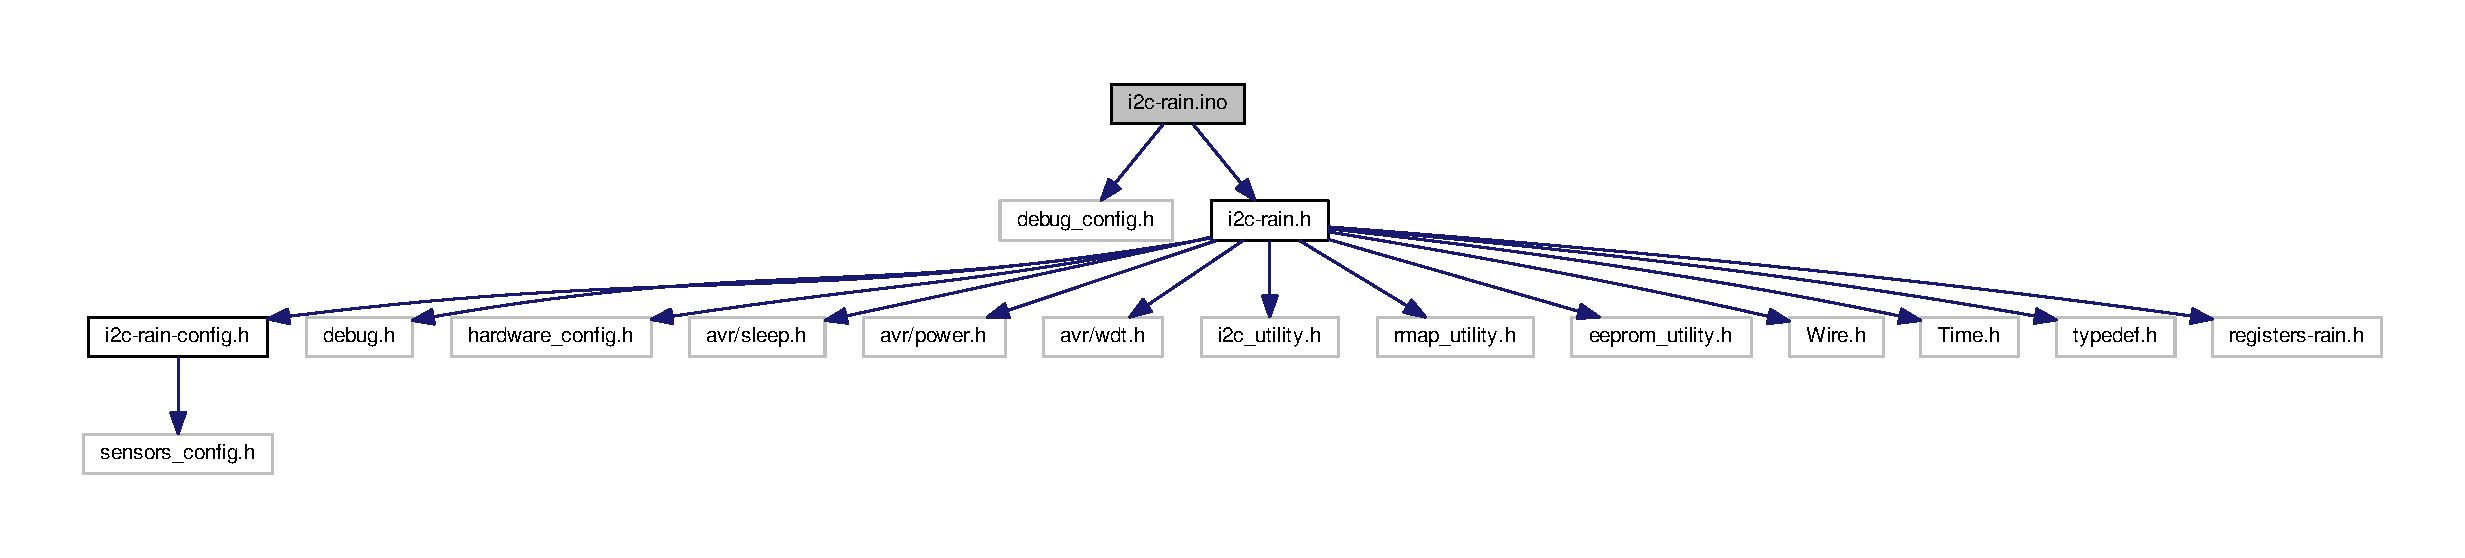
\includegraphics[width=350pt]{i2c-rain_8ino__incl}
\end{center}
\end{figure}
\subsection*{Macros}
\begin{DoxyCompactItemize}
\item 
\mbox{\Hypertarget{i2c-rain_8ino_a31fa5c36fa17c66feec7a67b76c3e786}\label{i2c-rain_8ino_a31fa5c36fa17c66feec7a67b76c3e786}} 
\#define \hyperlink{i2c-rain_8ino_a31fa5c36fa17c66feec7a67b76c3e786}{S\+E\+R\+I\+A\+L\+\_\+\+T\+R\+A\+C\+E\+\_\+\+L\+E\+V\+EL}~I2\+C\+\_\+\+R\+A\+I\+N\+\_\+\+S\+E\+R\+I\+A\+L\+\_\+\+T\+R\+A\+C\+E\+\_\+\+L\+E\+V\+EL
\begin{DoxyCompactList}\small\item\em Serial debug level for this sketch. \end{DoxyCompactList}\end{DoxyCompactItemize}
\subsection*{Functions}
\begin{DoxyCompactItemize}
\item 
void \hyperlink{i2c-rain_8ino_a4fc01d736fe50cf5b977f755b675f11d}{setup} ()
\begin{DoxyCompactList}\small\item\em Arduino setup function. Init watchdog, hardware, debug, buffer and load configuration stored in E\+E\+P\+R\+OM. \end{DoxyCompactList}\item 
void \hyperlink{i2c-rain_8ino_afe461d27b9c48d5921c00d521181f12f}{loop} ()
\begin{DoxyCompactList}\small\item\em Arduino loop function. First, initialize tasks and sensors, then execute the tasks and activates the power down if no task is running. \end{DoxyCompactList}\item 
void \hyperlink{i2c-rain_8ino_afb98a0f07c30784284f48271ffe02b97}{init\+\_\+power\+\_\+down} (uint32\+\_\+t $\ast$time\+\_\+ms, uint32\+\_\+t debouncing\+\_\+ms)
\begin{DoxyCompactList}\small\item\em Enter power down mode. \end{DoxyCompactList}\item 
void \hyperlink{i2c-rain_8ino_a980e73df66b14b1190bc25da430a4f12}{init\+\_\+wdt} (uint8\+\_\+t wdt\+\_\+timer)
\begin{DoxyCompactList}\small\item\em Init watchdog. \end{DoxyCompactList}\item 
void \hyperlink{i2c-rain_8ino_ad241cc00b1a92e6d85827df96778e442}{init\+\_\+buffers} ()
\begin{DoxyCompactList}\small\item\em Init buffers. \end{DoxyCompactList}\item 
void \hyperlink{i2c-rain_8ino_ab4bf0a3d77da083f131d3fa35a37d2b1}{init\+\_\+tasks} ()
\begin{DoxyCompactList}\small\item\em Init tasks variable and state. \end{DoxyCompactList}\item 
void \hyperlink{i2c-rain_8ino_ad8b80a0c08f928106018edd6ea435b95}{init\+\_\+pins} ()
\begin{DoxyCompactList}\small\item\em Init hardware pins. \end{DoxyCompactList}\item 
void \hyperlink{i2c-rain_8ino_a2441543100bf8421f56edd622a2c1d9a}{init\+\_\+wire} ()
\begin{DoxyCompactList}\small\item\em Init wire (i2c) library and performs checks on the bus. \end{DoxyCompactList}\item 
void \hyperlink{i2c-rain_8ino_a8eb9780a3438ec02c70314744f91f3c7}{init\+\_\+spi} ()
\begin{DoxyCompactList}\small\item\em Init S\+PI library. \end{DoxyCompactList}\item 
void \hyperlink{i2c-rain_8ino_ab985cc69f5f573113405b4f118c96d33}{init\+\_\+rtc} ()
\begin{DoxyCompactList}\small\item\em Init R\+TC module. \end{DoxyCompactList}\item 
void \hyperlink{i2c-rain_8ino_afceb890a6ab9be73cc5481369538c705}{init\+\_\+system} ()
\begin{DoxyCompactList}\small\item\em Init system. \end{DoxyCompactList}\item 
void \hyperlink{i2c-rain_8ino_ac74850003fab6eb3269bfe043d0f939c}{init\+\_\+sensors} ()
\begin{DoxyCompactList}\small\item\em Create and setup sensors. \end{DoxyCompactList}\item 
void \hyperlink{i2c-rain_8ino_a65b2dadc0411e43874ec8ed7f73bc62a}{print\+\_\+configuration} ()
\begin{DoxyCompactList}\small\item\em Print current configuration. \end{DoxyCompactList}\item 
void \hyperlink{i2c-rain_8ino_afa979a8cb238fe81bf20654dfd6096ef}{save\+\_\+configuration} (bool is\+\_\+default)
\begin{DoxyCompactList}\small\item\em Save configuration to E\+E\+P\+R\+OM. \end{DoxyCompactList}\item 
void \hyperlink{i2c-rain_8ino_a32a64a2800c724fb28e10636f2ec20b9}{load\+\_\+configuration} ()
\begin{DoxyCompactList}\small\item\em Load configuration from E\+E\+P\+R\+OM. \end{DoxyCompactList}\item 
void \hyperlink{i2c-rain_8ino_a368e45fb147aecb0fd1478d3cc76fba7}{tipping\+\_\+bucket\+\_\+interrupt\+\_\+handler} ()
\begin{DoxyCompactList}\small\item\em Tipping bucket interrupt handler. \end{DoxyCompactList}\item 
void \hyperlink{i2c-rain_8ino_ac816bd8aafe77e7a571574c8a26eead5}{i2c\+\_\+request\+\_\+interrupt\+\_\+handler} ()
\begin{DoxyCompactList}\small\item\em I2C request interrupt handler. \end{DoxyCompactList}\item 
void \hyperlink{i2c-rain_8ino_a6e27532df66f6bf186654355def5c9af}{i2c\+\_\+receive\+\_\+interrupt\+\_\+handler} (int rx\+\_\+data\+\_\+length)
\item 
void \hyperlink{i2c-rain_8ino_a009edfb36e6432603ed0ede845e2c12d}{tipping\+\_\+bucket\+\_\+task} ()
\begin{DoxyCompactList}\small\item\em Tipping bucket task. \end{DoxyCompactList}\item 
void \hyperlink{i2c-rain_8ino_a46696a96b3118b5d8900703c054166c8}{exchange\+\_\+buffers} ()
\begin{DoxyCompactList}\small\item\em Exchange reader and writer pointer to buffer. \end{DoxyCompactList}\item 
void \hyperlink{i2c-rain_8ino_a07daf3835b622d4d3451690f603845c1}{reset\+\_\+buffers} ()
\begin{DoxyCompactList}\small\item\em Reset buffers to default value. \end{DoxyCompactList}\item 
void \hyperlink{i2c-rain_8ino_a42389aceb96a84573eb67e6d141cb594}{command\+\_\+task} ()
\begin{DoxyCompactList}\small\item\em Execute the command received on i2c bus by reading i2c received data buffer. \end{DoxyCompactList}\item 
void \hyperlink{i2c-rain_8ino_a4981066e183f1432ffd6eddf55826585}{commands} ()
\begin{DoxyCompactList}\small\item\em Performs specific operations based on the received command. \end{DoxyCompactList}\end{DoxyCompactItemize}


\subsection{Function Documentation}
\mbox{\Hypertarget{i2c-rain_8ino_a42389aceb96a84573eb67e6d141cb594}\label{i2c-rain_8ino_a42389aceb96a84573eb67e6d141cb594}} 
\index{i2c-\/rain.\+ino@{i2c-\/rain.\+ino}!command\+\_\+task@{command\+\_\+task}}
\index{command\+\_\+task@{command\+\_\+task}!i2c-\/rain.\+ino@{i2c-\/rain.\+ino}}
\subsubsection{\texorpdfstring{command\+\_\+task()}{command\_task()}}
{\footnotesize\ttfamily void command\+\_\+task (\begin{DoxyParamCaption}\item[{void}]{ }\end{DoxyParamCaption})}



Execute the command received on i2c bus by reading i2c received data buffer. 

\begin{DoxyReturn}{Returns}
void. 
\end{DoxyReturn}
\mbox{\Hypertarget{i2c-rain_8ino_a4981066e183f1432ffd6eddf55826585}\label{i2c-rain_8ino_a4981066e183f1432ffd6eddf55826585}} 
\index{i2c-\/rain.\+ino@{i2c-\/rain.\+ino}!commands@{commands}}
\index{commands@{commands}!i2c-\/rain.\+ino@{i2c-\/rain.\+ino}}
\subsubsection{\texorpdfstring{commands()}{commands()}}
{\footnotesize\ttfamily void commands (\begin{DoxyParamCaption}\item[{void}]{ }\end{DoxyParamCaption})}



Performs specific operations based on the received command. 

\begin{DoxyReturn}{Returns}
void. 
\end{DoxyReturn}
\mbox{\Hypertarget{i2c-rain_8ino_a46696a96b3118b5d8900703c054166c8}\label{i2c-rain_8ino_a46696a96b3118b5d8900703c054166c8}} 
\index{i2c-\/rain.\+ino@{i2c-\/rain.\+ino}!exchange\+\_\+buffers@{exchange\+\_\+buffers}}
\index{exchange\+\_\+buffers@{exchange\+\_\+buffers}!i2c-\/rain.\+ino@{i2c-\/rain.\+ino}}
\subsubsection{\texorpdfstring{exchange\+\_\+buffers()}{exchange\_buffers()}}
{\footnotesize\ttfamily void exchange\+\_\+buffers (\begin{DoxyParamCaption}\item[{void}]{ }\end{DoxyParamCaption})}



Exchange reader and writer pointer to buffer. 

\begin{DoxyReturn}{Returns}
void. 
\end{DoxyReturn}
\mbox{\Hypertarget{i2c-rain_8ino_a6e27532df66f6bf186654355def5c9af}\label{i2c-rain_8ino_a6e27532df66f6bf186654355def5c9af}} 
\index{i2c-\/rain.\+ino@{i2c-\/rain.\+ino}!i2c\+\_\+receive\+\_\+interrupt\+\_\+handler@{i2c\+\_\+receive\+\_\+interrupt\+\_\+handler}}
\index{i2c\+\_\+receive\+\_\+interrupt\+\_\+handler@{i2c\+\_\+receive\+\_\+interrupt\+\_\+handler}!i2c-\/rain.\+ino@{i2c-\/rain.\+ino}}
\subsubsection{\texorpdfstring{i2c\+\_\+receive\+\_\+interrupt\+\_\+handler()}{i2c\_receive\_interrupt\_handler()}}
{\footnotesize\ttfamily void i2c\+\_\+receive\+\_\+interrupt\+\_\+handler (\begin{DoxyParamCaption}\item[{int}]{rx\+\_\+data\+\_\+length }\end{DoxyParamCaption})}

read rx\+\_\+data\+\_\+length bytes of data from i2c bus

it is a registers read?

offset in readable\+\_\+data\+\_\+read\+\_\+ptr buffer

length (in butes) of data to be read in readable\+\_\+data\+\_\+read\+\_\+ptr

it is a command?

enable Command task

it is a registers write?

write rx\+\_\+data\+\_\+length bytes in writable\+\_\+data\+\_\+ptr (base) at (i2c\+\_\+rx\+\_\+data\mbox{[}i\mbox{]} -\/ I2\+C\+\_\+\+W\+R\+I\+T\+E\+\_\+\+R\+E\+G\+I\+S\+T\+E\+R\+\_\+\+S\+T\+A\+R\+T\+\_\+\+A\+D\+D\+R\+E\+SS) (position in buffer) \mbox{\Hypertarget{i2c-rain_8ino_ac816bd8aafe77e7a571574c8a26eead5}\label{i2c-rain_8ino_ac816bd8aafe77e7a571574c8a26eead5}} 
\index{i2c-\/rain.\+ino@{i2c-\/rain.\+ino}!i2c\+\_\+request\+\_\+interrupt\+\_\+handler@{i2c\+\_\+request\+\_\+interrupt\+\_\+handler}}
\index{i2c\+\_\+request\+\_\+interrupt\+\_\+handler@{i2c\+\_\+request\+\_\+interrupt\+\_\+handler}!i2c-\/rain.\+ino@{i2c-\/rain.\+ino}}
\subsubsection{\texorpdfstring{i2c\+\_\+request\+\_\+interrupt\+\_\+handler()}{i2c\_request\_interrupt\_handler()}}
{\footnotesize\ttfamily void i2c\+\_\+request\+\_\+interrupt\+\_\+handler (\begin{DoxyParamCaption}\item[{void}]{ }\end{DoxyParamCaption})}



I2C request interrupt handler. 

\begin{DoxyReturn}{Returns}
void. 
\end{DoxyReturn}
write readable\+\_\+data\+\_\+length bytes of data stored in readable\+\_\+data\+\_\+read\+\_\+ptr (base) + readable\+\_\+data\+\_\+address (offset) on i2c bus \mbox{\Hypertarget{i2c-rain_8ino_ad241cc00b1a92e6d85827df96778e442}\label{i2c-rain_8ino_ad241cc00b1a92e6d85827df96778e442}} 
\index{i2c-\/rain.\+ino@{i2c-\/rain.\+ino}!init\+\_\+buffers@{init\+\_\+buffers}}
\index{init\+\_\+buffers@{init\+\_\+buffers}!i2c-\/rain.\+ino@{i2c-\/rain.\+ino}}
\subsubsection{\texorpdfstring{init\+\_\+buffers()}{init\_buffers()}}
{\footnotesize\ttfamily void init\+\_\+buffers (\begin{DoxyParamCaption}\item[{void}]{ }\end{DoxyParamCaption})}



Init buffers. 

\begin{DoxyReturn}{Returns}
void. 
\end{DoxyReturn}
copy readable\+\_\+data\+\_\+2 in readable\+\_\+data\+\_\+1 \mbox{\Hypertarget{i2c-rain_8ino_ad8b80a0c08f928106018edd6ea435b95}\label{i2c-rain_8ino_ad8b80a0c08f928106018edd6ea435b95}} 
\index{i2c-\/rain.\+ino@{i2c-\/rain.\+ino}!init\+\_\+pins@{init\+\_\+pins}}
\index{init\+\_\+pins@{init\+\_\+pins}!i2c-\/rain.\+ino@{i2c-\/rain.\+ino}}
\subsubsection{\texorpdfstring{init\+\_\+pins()}{init\_pins()}}
{\footnotesize\ttfamily void init\+\_\+pins (\begin{DoxyParamCaption}\item[{void}]{ }\end{DoxyParamCaption})}



Init hardware pins. 

\begin{DoxyReturn}{Returns}
void. 
\end{DoxyReturn}
\mbox{\Hypertarget{i2c-rain_8ino_afb98a0f07c30784284f48271ffe02b97}\label{i2c-rain_8ino_afb98a0f07c30784284f48271ffe02b97}} 
\index{i2c-\/rain.\+ino@{i2c-\/rain.\+ino}!init\+\_\+power\+\_\+down@{init\+\_\+power\+\_\+down}}
\index{init\+\_\+power\+\_\+down@{init\+\_\+power\+\_\+down}!i2c-\/rain.\+ino@{i2c-\/rain.\+ino}}
\subsubsection{\texorpdfstring{init\+\_\+power\+\_\+down()}{init\_power\_down()}}
{\footnotesize\ttfamily void init\+\_\+power\+\_\+down (\begin{DoxyParamCaption}\item[{uint32\+\_\+t $\ast$}]{time\+\_\+ms,  }\item[{uint32\+\_\+t}]{debouncing\+\_\+ms }\end{DoxyParamCaption})}



Enter power down mode. 


\begin{DoxyParams}{Parameters}
{\em time\+\_\+ms} & pointer to a variable to save the last instant you entered power down. \\
\hline
{\em debouncing\+\_\+ms} & delay to power down. \\
\hline
\end{DoxyParams}
\begin{DoxyReturn}{Returns}
void. 
\end{DoxyReturn}
turn off brown-\/out \mbox{\Hypertarget{i2c-rain_8ino_ab985cc69f5f573113405b4f118c96d33}\label{i2c-rain_8ino_ab985cc69f5f573113405b4f118c96d33}} 
\index{i2c-\/rain.\+ino@{i2c-\/rain.\+ino}!init\+\_\+rtc@{init\+\_\+rtc}}
\index{init\+\_\+rtc@{init\+\_\+rtc}!i2c-\/rain.\+ino@{i2c-\/rain.\+ino}}
\subsubsection{\texorpdfstring{init\+\_\+rtc()}{init\_rtc()}}
{\footnotesize\ttfamily void init\+\_\+rtc (\begin{DoxyParamCaption}\item[{void}]{ }\end{DoxyParamCaption})}



Init R\+TC module. 

\begin{DoxyReturn}{Returns}
void. 
\end{DoxyReturn}
\mbox{\Hypertarget{i2c-rain_8ino_ac74850003fab6eb3269bfe043d0f939c}\label{i2c-rain_8ino_ac74850003fab6eb3269bfe043d0f939c}} 
\index{i2c-\/rain.\+ino@{i2c-\/rain.\+ino}!init\+\_\+sensors@{init\+\_\+sensors}}
\index{init\+\_\+sensors@{init\+\_\+sensors}!i2c-\/rain.\+ino@{i2c-\/rain.\+ino}}
\subsubsection{\texorpdfstring{init\+\_\+sensors()}{init\_sensors()}}
{\footnotesize\ttfamily void init\+\_\+sensors (\begin{DoxyParamCaption}\item[{void}]{ }\end{DoxyParamCaption})}



Create and setup sensors. 

\begin{DoxyReturn}{Returns}
void. 
\end{DoxyReturn}
\mbox{\Hypertarget{i2c-rain_8ino_a8eb9780a3438ec02c70314744f91f3c7}\label{i2c-rain_8ino_a8eb9780a3438ec02c70314744f91f3c7}} 
\index{i2c-\/rain.\+ino@{i2c-\/rain.\+ino}!init\+\_\+spi@{init\+\_\+spi}}
\index{init\+\_\+spi@{init\+\_\+spi}!i2c-\/rain.\+ino@{i2c-\/rain.\+ino}}
\subsubsection{\texorpdfstring{init\+\_\+spi()}{init\_spi()}}
{\footnotesize\ttfamily void init\+\_\+spi (\begin{DoxyParamCaption}\item[{void}]{ }\end{DoxyParamCaption})}



Init S\+PI library. 

\begin{DoxyReturn}{Returns}
void. 
\end{DoxyReturn}
\mbox{\Hypertarget{i2c-rain_8ino_afceb890a6ab9be73cc5481369538c705}\label{i2c-rain_8ino_afceb890a6ab9be73cc5481369538c705}} 
\index{i2c-\/rain.\+ino@{i2c-\/rain.\+ino}!init\+\_\+system@{init\+\_\+system}}
\index{init\+\_\+system@{init\+\_\+system}!i2c-\/rain.\+ino@{i2c-\/rain.\+ino}}
\subsubsection{\texorpdfstring{init\+\_\+system()}{init\_system()}}
{\footnotesize\ttfamily void init\+\_\+system (\begin{DoxyParamCaption}\item[{void}]{ }\end{DoxyParamCaption})}



Init system. 

\begin{DoxyReturn}{Returns}
void. 
\end{DoxyReturn}
main loop state \mbox{\Hypertarget{i2c-rain_8ino_ab4bf0a3d77da083f131d3fa35a37d2b1}\label{i2c-rain_8ino_ab4bf0a3d77da083f131d3fa35a37d2b1}} 
\index{i2c-\/rain.\+ino@{i2c-\/rain.\+ino}!init\+\_\+tasks@{init\+\_\+tasks}}
\index{init\+\_\+tasks@{init\+\_\+tasks}!i2c-\/rain.\+ino@{i2c-\/rain.\+ino}}
\subsubsection{\texorpdfstring{init\+\_\+tasks()}{init\_tasks()}}
{\footnotesize\ttfamily void init\+\_\+tasks (\begin{DoxyParamCaption}\item[{void}]{ }\end{DoxyParamCaption})}



Init tasks variable and state. 

\begin{DoxyReturn}{Returns}
void. 
\end{DoxyReturn}
no tasks ready

reset tipping bucket debounce value \mbox{\Hypertarget{i2c-rain_8ino_a980e73df66b14b1190bc25da430a4f12}\label{i2c-rain_8ino_a980e73df66b14b1190bc25da430a4f12}} 
\index{i2c-\/rain.\+ino@{i2c-\/rain.\+ino}!init\+\_\+wdt@{init\+\_\+wdt}}
\index{init\+\_\+wdt@{init\+\_\+wdt}!i2c-\/rain.\+ino@{i2c-\/rain.\+ino}}
\subsubsection{\texorpdfstring{init\+\_\+wdt()}{init\_wdt()}}
{\footnotesize\ttfamily void init\+\_\+wdt (\begin{DoxyParamCaption}\item[{uint8\+\_\+t}]{wdt\+\_\+timer }\end{DoxyParamCaption})}



Init watchdog. 


\begin{DoxyParams}{Parameters}
{\em wdt\+\_\+timer} & a time value for init watchdog (W\+D\+T\+O\+\_\+xxxx). \\
\hline
\end{DoxyParams}
\begin{DoxyReturn}{Returns}
void. 
\end{DoxyReturn}
\mbox{\Hypertarget{i2c-rain_8ino_a2441543100bf8421f56edd622a2c1d9a}\label{i2c-rain_8ino_a2441543100bf8421f56edd622a2c1d9a}} 
\index{i2c-\/rain.\+ino@{i2c-\/rain.\+ino}!init\+\_\+wire@{init\+\_\+wire}}
\index{init\+\_\+wire@{init\+\_\+wire}!i2c-\/rain.\+ino@{i2c-\/rain.\+ino}}
\subsubsection{\texorpdfstring{init\+\_\+wire()}{init\_wire()}}
{\footnotesize\ttfamily void init\+\_\+wire (\begin{DoxyParamCaption}\item[{void}]{ }\end{DoxyParamCaption})}



Init wire (i2c) library and performs checks on the bus. 

\begin{DoxyReturn}{Returns}
void. 
\end{DoxyReturn}
clear the I2C bus first before calling Wire.\+begin()

wait for watchdog reboot \mbox{\Hypertarget{i2c-rain_8ino_a32a64a2800c724fb28e10636f2ec20b9}\label{i2c-rain_8ino_a32a64a2800c724fb28e10636f2ec20b9}} 
\index{i2c-\/rain.\+ino@{i2c-\/rain.\+ino}!load\+\_\+configuration@{load\+\_\+configuration}}
\index{load\+\_\+configuration@{load\+\_\+configuration}!i2c-\/rain.\+ino@{i2c-\/rain.\+ino}}
\subsubsection{\texorpdfstring{load\+\_\+configuration()}{load\_configuration()}}
{\footnotesize\ttfamily void load\+\_\+configuration (\begin{DoxyParamCaption}\item[{void}]{ }\end{DoxyParamCaption})}



Load configuration from E\+E\+P\+R\+OM. 

\begin{DoxyReturn}{Returns}
void. 
\end{DoxyReturn}
read configuration from eeprom

set configuration value to writable register \mbox{\Hypertarget{i2c-rain_8ino_afe461d27b9c48d5921c00d521181f12f}\label{i2c-rain_8ino_afe461d27b9c48d5921c00d521181f12f}} 
\index{i2c-\/rain.\+ino@{i2c-\/rain.\+ino}!loop@{loop}}
\index{loop@{loop}!i2c-\/rain.\+ino@{i2c-\/rain.\+ino}}
\subsubsection{\texorpdfstring{loop()}{loop()}}
{\footnotesize\ttfamily void loop (\begin{DoxyParamCaption}{ }\end{DoxyParamCaption})}



Arduino loop function. First, initialize tasks and sensors, then execute the tasks and activates the power down if no task is running. 

\begin{DoxyReturn}{Returns}
void. 
\end{DoxyReturn}
\mbox{\Hypertarget{i2c-rain_8ino_a65b2dadc0411e43874ec8ed7f73bc62a}\label{i2c-rain_8ino_a65b2dadc0411e43874ec8ed7f73bc62a}} 
\index{i2c-\/rain.\+ino@{i2c-\/rain.\+ino}!print\+\_\+configuration@{print\+\_\+configuration}}
\index{print\+\_\+configuration@{print\+\_\+configuration}!i2c-\/rain.\+ino@{i2c-\/rain.\+ino}}
\subsubsection{\texorpdfstring{print\+\_\+configuration()}{print\_configuration()}}
{\footnotesize\ttfamily void print\+\_\+configuration (\begin{DoxyParamCaption}\item[{void}]{ }\end{DoxyParamCaption})}



Print current configuration. 

\begin{DoxyReturn}{Returns}
void. 
\end{DoxyReturn}
\mbox{\Hypertarget{i2c-rain_8ino_a07daf3835b622d4d3451690f603845c1}\label{i2c-rain_8ino_a07daf3835b622d4d3451690f603845c1}} 
\index{i2c-\/rain.\+ino@{i2c-\/rain.\+ino}!reset\+\_\+buffers@{reset\+\_\+buffers}}
\index{reset\+\_\+buffers@{reset\+\_\+buffers}!i2c-\/rain.\+ino@{i2c-\/rain.\+ino}}
\subsubsection{\texorpdfstring{reset\+\_\+buffers()}{reset\_buffers()}}
{\footnotesize\ttfamily void reset\+\_\+buffers (\begin{DoxyParamCaption}\item[{void}]{ }\end{DoxyParamCaption})}



Reset buffers to default value. 

\begin{DoxyReturn}{Returns}
void. 
\end{DoxyReturn}
\mbox{\Hypertarget{i2c-rain_8ino_afa979a8cb238fe81bf20654dfd6096ef}\label{i2c-rain_8ino_afa979a8cb238fe81bf20654dfd6096ef}} 
\index{i2c-\/rain.\+ino@{i2c-\/rain.\+ino}!save\+\_\+configuration@{save\+\_\+configuration}}
\index{save\+\_\+configuration@{save\+\_\+configuration}!i2c-\/rain.\+ino@{i2c-\/rain.\+ino}}
\subsubsection{\texorpdfstring{save\+\_\+configuration()}{save\_configuration()}}
{\footnotesize\ttfamily void save\+\_\+configuration (\begin{DoxyParamCaption}\item[{bool}]{is\+\_\+default }\end{DoxyParamCaption})}



Save configuration to E\+E\+P\+R\+OM. 


\begin{DoxyParams}{Parameters}
{\em is\+\_\+default} & if true save default configuration; if false save current configuration. \\
\hline
\end{DoxyParams}
\begin{DoxyReturn}{Returns}
void. 
\end{DoxyReturn}
write configuration to eeprom \mbox{\Hypertarget{i2c-rain_8ino_a4fc01d736fe50cf5b977f755b675f11d}\label{i2c-rain_8ino_a4fc01d736fe50cf5b977f755b675f11d}} 
\index{i2c-\/rain.\+ino@{i2c-\/rain.\+ino}!setup@{setup}}
\index{setup@{setup}!i2c-\/rain.\+ino@{i2c-\/rain.\+ino}}
\subsubsection{\texorpdfstring{setup()}{setup()}}
{\footnotesize\ttfamily void setup (\begin{DoxyParamCaption}{ }\end{DoxyParamCaption})}



Arduino setup function. Init watchdog, hardware, debug, buffer and load configuration stored in E\+E\+P\+R\+OM. 

\begin{DoxyReturn}{Returns}
void. 
\end{DoxyReturn}
\mbox{\Hypertarget{i2c-rain_8ino_a368e45fb147aecb0fd1478d3cc76fba7}\label{i2c-rain_8ino_a368e45fb147aecb0fd1478d3cc76fba7}} 
\index{i2c-\/rain.\+ino@{i2c-\/rain.\+ino}!tipping\+\_\+bucket\+\_\+interrupt\+\_\+handler@{tipping\+\_\+bucket\+\_\+interrupt\+\_\+handler}}
\index{tipping\+\_\+bucket\+\_\+interrupt\+\_\+handler@{tipping\+\_\+bucket\+\_\+interrupt\+\_\+handler}!i2c-\/rain.\+ino@{i2c-\/rain.\+ino}}
\subsubsection{\texorpdfstring{tipping\+\_\+bucket\+\_\+interrupt\+\_\+handler()}{tipping\_bucket\_interrupt\_handler()}}
{\footnotesize\ttfamily void tipping\+\_\+bucket\+\_\+interrupt\+\_\+handler (\begin{DoxyParamCaption}\item[{void}]{ }\end{DoxyParamCaption})}



Tipping bucket interrupt handler. 

\begin{DoxyReturn}{Returns}
void. 
\end{DoxyReturn}
reading T\+I\+P\+P\+I\+N\+G\+\_\+\+B\+U\+C\+K\+E\+T\+\_\+\+P\+IN value to be sure the interrupt has occurred

enable Tipping bucket task \mbox{\Hypertarget{i2c-rain_8ino_a009edfb36e6432603ed0ede845e2c12d}\label{i2c-rain_8ino_a009edfb36e6432603ed0ede845e2c12d}} 
\index{i2c-\/rain.\+ino@{i2c-\/rain.\+ino}!tipping\+\_\+bucket\+\_\+task@{tipping\+\_\+bucket\+\_\+task}}
\index{tipping\+\_\+bucket\+\_\+task@{tipping\+\_\+bucket\+\_\+task}!i2c-\/rain.\+ino@{i2c-\/rain.\+ino}}
\subsubsection{\texorpdfstring{tipping\+\_\+bucket\+\_\+task()}{tipping\_bucket\_task()}}
{\footnotesize\ttfamily void tipping\+\_\+bucket\+\_\+task (\begin{DoxyParamCaption}\item[{void}]{ }\end{DoxyParamCaption})}



Tipping bucket task. 

\begin{DoxyReturn}{Returns}
void. 
\end{DoxyReturn}
check if last tipping bucket event has happened for more than D\+E\+B\+O\+U\+N\+C\+I\+N\+G\+\_\+\+T\+I\+P\+P\+I\+N\+G\+\_\+\+B\+U\+C\+K\+E\+T\+\_\+\+T\+I\+M\+E\+\_\+\+MS ms

increment rain tips if oneshot mode is on and oneshot start command It has been received 
%--- End generated contents ---

% Index
\backmatter
\newpage
\phantomsection
\clearemptydoublepage
\addcontentsline{toc}{chapter}{Index}
\printindex

\end{document}
